% Options for packages loaded elsewhere
\PassOptionsToPackage{unicode}{hyperref}
\PassOptionsToPackage{hyphens}{url}
%
\documentclass[
]{article}
\usepackage{amsmath,amssymb}
\usepackage{iftex}
\ifPDFTeX
  \usepackage[T1]{fontenc}
  \usepackage[utf8]{inputenc}
  \usepackage{textcomp} % provide euro and other symbols
\else % if luatex or xetex
  \usepackage{unicode-math} % this also loads fontspec
  \defaultfontfeatures{Scale=MatchLowercase}
  \defaultfontfeatures[\rmfamily]{Ligatures=TeX,Scale=1}
\fi
\usepackage{lmodern}
\ifPDFTeX\else
  % xetex/luatex font selection
\fi
% Use upquote if available, for straight quotes in verbatim environments
\IfFileExists{upquote.sty}{\usepackage{upquote}}{}
\IfFileExists{microtype.sty}{% use microtype if available
  \usepackage[]{microtype}
  \UseMicrotypeSet[protrusion]{basicmath} % disable protrusion for tt fonts
}{}
\makeatletter
\@ifundefined{KOMAClassName}{% if non-KOMA class
  \IfFileExists{parskip.sty}{%
    \usepackage{parskip}
  }{% else
    \setlength{\parindent}{0pt}
    \setlength{\parskip}{6pt plus 2pt minus 1pt}}
}{% if KOMA class
  \KOMAoptions{parskip=half}}
\makeatother
\usepackage{xcolor}
\usepackage[margin=1in]{geometry}
\usepackage{color}
\usepackage{fancyvrb}
\newcommand{\VerbBar}{|}
\newcommand{\VERB}{\Verb[commandchars=\\\{\}]}
\DefineVerbatimEnvironment{Highlighting}{Verbatim}{commandchars=\\\{\}}
% Add ',fontsize=\small' for more characters per line
\usepackage{framed}
\definecolor{shadecolor}{RGB}{248,248,248}
\newenvironment{Shaded}{\begin{snugshade}}{\end{snugshade}}
\newcommand{\AlertTok}[1]{\textcolor[rgb]{0.94,0.16,0.16}{#1}}
\newcommand{\AnnotationTok}[1]{\textcolor[rgb]{0.56,0.35,0.01}{\textbf{\textit{#1}}}}
\newcommand{\AttributeTok}[1]{\textcolor[rgb]{0.13,0.29,0.53}{#1}}
\newcommand{\BaseNTok}[1]{\textcolor[rgb]{0.00,0.00,0.81}{#1}}
\newcommand{\BuiltInTok}[1]{#1}
\newcommand{\CharTok}[1]{\textcolor[rgb]{0.31,0.60,0.02}{#1}}
\newcommand{\CommentTok}[1]{\textcolor[rgb]{0.56,0.35,0.01}{\textit{#1}}}
\newcommand{\CommentVarTok}[1]{\textcolor[rgb]{0.56,0.35,0.01}{\textbf{\textit{#1}}}}
\newcommand{\ConstantTok}[1]{\textcolor[rgb]{0.56,0.35,0.01}{#1}}
\newcommand{\ControlFlowTok}[1]{\textcolor[rgb]{0.13,0.29,0.53}{\textbf{#1}}}
\newcommand{\DataTypeTok}[1]{\textcolor[rgb]{0.13,0.29,0.53}{#1}}
\newcommand{\DecValTok}[1]{\textcolor[rgb]{0.00,0.00,0.81}{#1}}
\newcommand{\DocumentationTok}[1]{\textcolor[rgb]{0.56,0.35,0.01}{\textbf{\textit{#1}}}}
\newcommand{\ErrorTok}[1]{\textcolor[rgb]{0.64,0.00,0.00}{\textbf{#1}}}
\newcommand{\ExtensionTok}[1]{#1}
\newcommand{\FloatTok}[1]{\textcolor[rgb]{0.00,0.00,0.81}{#1}}
\newcommand{\FunctionTok}[1]{\textcolor[rgb]{0.13,0.29,0.53}{\textbf{#1}}}
\newcommand{\ImportTok}[1]{#1}
\newcommand{\InformationTok}[1]{\textcolor[rgb]{0.56,0.35,0.01}{\textbf{\textit{#1}}}}
\newcommand{\KeywordTok}[1]{\textcolor[rgb]{0.13,0.29,0.53}{\textbf{#1}}}
\newcommand{\NormalTok}[1]{#1}
\newcommand{\OperatorTok}[1]{\textcolor[rgb]{0.81,0.36,0.00}{\textbf{#1}}}
\newcommand{\OtherTok}[1]{\textcolor[rgb]{0.56,0.35,0.01}{#1}}
\newcommand{\PreprocessorTok}[1]{\textcolor[rgb]{0.56,0.35,0.01}{\textit{#1}}}
\newcommand{\RegionMarkerTok}[1]{#1}
\newcommand{\SpecialCharTok}[1]{\textcolor[rgb]{0.81,0.36,0.00}{\textbf{#1}}}
\newcommand{\SpecialStringTok}[1]{\textcolor[rgb]{0.31,0.60,0.02}{#1}}
\newcommand{\StringTok}[1]{\textcolor[rgb]{0.31,0.60,0.02}{#1}}
\newcommand{\VariableTok}[1]{\textcolor[rgb]{0.00,0.00,0.00}{#1}}
\newcommand{\VerbatimStringTok}[1]{\textcolor[rgb]{0.31,0.60,0.02}{#1}}
\newcommand{\WarningTok}[1]{\textcolor[rgb]{0.56,0.35,0.01}{\textbf{\textit{#1}}}}
\usepackage{graphicx}
\makeatletter
\def\maxwidth{\ifdim\Gin@nat@width>\linewidth\linewidth\else\Gin@nat@width\fi}
\def\maxheight{\ifdim\Gin@nat@height>\textheight\textheight\else\Gin@nat@height\fi}
\makeatother
% Scale images if necessary, so that they will not overflow the page
% margins by default, and it is still possible to overwrite the defaults
% using explicit options in \includegraphics[width, height, ...]{}
\setkeys{Gin}{width=\maxwidth,height=\maxheight,keepaspectratio}
% Set default figure placement to htbp
\makeatletter
\def\fps@figure{htbp}
\makeatother
\setlength{\emergencystretch}{3em} % prevent overfull lines
\providecommand{\tightlist}{%
  \setlength{\itemsep}{0pt}\setlength{\parskip}{0pt}}
\setcounter{secnumdepth}{-\maxdimen} % remove section numbering
\usepackage{booktabs}
\usepackage{longtable}
\usepackage{array}
\usepackage{multirow}
\usepackage{wrapfig}
\usepackage{float}
\usepackage{colortbl}
\usepackage{pdflscape}
\usepackage{tabu}
\usepackage{threeparttable}
\usepackage{threeparttablex}
\usepackage[normalem]{ulem}
\usepackage{makecell}
\usepackage{xcolor}
\ifLuaTeX
  \usepackage{selnolig}  % disable illegal ligatures
\fi
\IfFileExists{bookmark.sty}{\usepackage{bookmark}}{\usepackage{hyperref}}
\IfFileExists{xurl.sty}{\usepackage{xurl}}{} % add URL line breaks if available
\urlstyle{same}
\hypersetup{
  pdftitle={Manuscript progress report},
  pdfauthor={Ying Jin},
  hidelinks,
  pdfcreator={LaTeX via pandoc}}

\title{Manuscript progress report}
\author{Ying Jin}
\date{2024-02-16}

\begin{document}
\maketitle

{
\setcounter{tocdepth}{3}
\tableofcontents
}
\hypertarget{method}{%
\section{Method}\label{method}}

\hypertarget{assumptions}{%
\subsection{Assumptions}\label{assumptions}}

\begin{itemize}
\tightlist
\item
  For each subject i in the population, a generalized outcome \(Y_i(t)\)
  is generated along a variable t (for example, time), where
  \(t \in (0, T)\).
\item
  The outcome, at any specific t, follows an exponential family
  distribution characterized by a (latent) continuous function
  \(\eta_i(t)\):
\end{itemize}

\[g[E(Y_i(t))] = \eta_i(t) = \beta_0(t)+b_i(t)\]

\[p(Y_i(t)) = h(Y_i(t))exp\{\eta_i(t)T[Y_i(t)]-A(\eta_i(t))\}\]

\begin{itemize}
\tightlist
\item
  The continuous latent function consists of a population-level fixed
  process and an individual-level random process
\end{itemize}

\[\eta_i(t) = \beta_0(t)+b_i(t)\]

\hypertarget{observed-data}{%
\subsection{Observed data}\label{observed-data}}

In practice we would observe the discrete realization of
\(\{Y_i(t), t\}\) along a dense grid. For simplicity, we assume the
observation grid is regular (same across sample). When we have J
observations points in \((0, T]\), then for the jth observation point,
we denote the corresponding value of t as \(t_j\), and the corresponding
outcome at this point \(Y_i(t_j)\).

\hypertarget{fgfpca-algorithm}{%
\subsection{fGFPCA Algorithm}\label{fgfpca-algorithm}}

\hypertarget{bin-data}{%
\subsubsection{Bin data:}\label{bin-data}}

Choose a proper bin width \(w\) considering model complexity and
identifiability. For now let's say the bins are equal-length and
non-overlapping.

\begin{itemize}
\tightlist
\item
  Bin index \(s = 1...S\)
\item
  Index of bin midpoints \(m_s\)
\item
  Value of t corresponding to bin midpoints \(t_{m_s}\)
\item
  Bin endpoints: \((t_{m_s}-\frac{w}{2}, t_{m_s}+\frac{w}{2}]\)
\end{itemize}

\hypertarget{local-glmms}{%
\subsubsection{Local GLMMs}\label{local-glmms}}

At the every bin, we fit a local intercept-only model:

\[g[E(Y_i(t_j))] =\eta_i(t_{m_s})= \beta_0(t_{m_s})+b_i(t_{m_s})\] where
\(t_j \in (t_{m_s}-\frac{w}{2}, t_{m_s}+\frac{w}{2}]\).

Here we are basically saying that the value of latent function is
constant within the same bin, which clearly is a misspecification of the
true latent process.

From the model above. we will be able to estimate a
\(\hat{\eta_i}(t_{m_s})\) on the binned grid for every individual in the
training sample.

\hypertarget{fpca}{%
\subsubsection{FPCA}\label{fpca}}

Here, we fit a FPCA model on the \(\hat{\eta_i}(t_{m_s})\) obtained from
step 2:

\[\hat{\eta}_i(t_{m_s}) = f_0(t_{m_s})+\sum_{k=1}^K\xi_{ik}\phi_{k}(t_{m_s})+\epsilon_i(t_{m_s})\]

where \(\xi_{ik}\) independently follows normal distribution
\(N(0, \lambda_k)\), and \(\epsilon_i(t_{m_s})\) at each point follows
\(N(0, \sigma_2)\).

From this model, we will be able to obtain the following estimates which
are shared across population:

\begin{itemize}
\tightlist
\item
  Population mean \(\hat{f_0}(t_{m_s})\)
\item
  Basis functions
  \(\hat{\mathbf{\Phi}} = \{\hat{\phi}_1(t_{m_s}), ...,\hat{\phi}_K(t_{m_s}))\}\)
\item
  Estimates of variance of scores \(\hat{\lambda}_1...\hat{\lambda}_K\)
\end{itemize}

\hypertarget{projection-and-debias}{%
\subsubsection{Projection and Debias}\label{projection-and-debias}}

The mean and basis functions are evaluated on the binned grid. To extend
it to the original measurement grid data was collected on, we project
the estimated eigenfunctions \(\hat{\mathbf{\Phi}}\) back use spline
basis. Now we have extend the \(\hat{\phi}_k(t_{m_s})\) to the original
grid \(\hat{\phi}_k(t_j)\)

Because of the misspecification of local GLMMs, the estimated
eigenfunctions and eigenvalues are also biased by a constant
multiplicative effect. Therefore, we use a GLMM to re-evaluate the mean
function, eigenfunctions and eigenvalues.

\hypertarget{out-of-sample-prediction}{%
\subsection{Out-of-sample prediction}\label{out-of-sample-prediction}}

Now, let's assume we have a new subject \(u\) with \(J_u\) observations
(\(J_u < J\)). Then the log-likelihood of this new subject would be:

\[l_u=\sum_{t_j<t_{J_u}}log(h(Y_u(t_j)))+\hat{\eta}_u(t_j)T(Y_u(t_j))-log(A[\hat{\eta}_u(t_j)])\]

where
\(\hat{\eta}_u(t_j) = \hat{f}_0(t_j)+\sum_{k=1}^K \xi_{uk}\hat{\phi}(t_j)\).

With estimates for the population-level parameters from fGFPCA
algorithms above, we can estimate \(\xi_{uk}\) by maximization of
\(l_u\). Direct maximization some times does not have closed form
solution. Numeric maximization methods seem not very stable as well. So
I have decided to used a Bayes approach (Laplace Approximation):

\begin{itemize}
\tightlist
\item
  Prior distribution: \(\xi_{uk} \sim N(0, \hat{\lambda}_k)\)
\item
  Posterior distribution: the likelihood of
  \(l_u =l(Y_u(t_j)|\mathbf{\xi}_u)\)
\end{itemize}

Laplace Approximation would get the posterior mode of \(\xi_{uk}\)
through quadratic approximation.

\hypertarget{reference-method}{%
\section{Reference method}\label{reference-method}}

\hypertarget{glmmadaptive}{%
\subsection{GLMMadaptive}\label{glmmadaptive}}

\begin{itemize}
\tightlist
\item
  For large datasets, we can fit a model with random intercept and slope
  for time. It is doable on 500 datasets, but obviously too simple for
  the data generation scheme. We would expect it to perform terribly.
\end{itemize}

\[g(E(Y_i(t))) = \beta_0+\beta_1t+b_{i0}+b_{i1}t\]

\begin{itemize}
\tightlist
\item
  For small datasets, we would like to fit fGFPCA and GLMMadaptive on a
  dataset with smaller sample size and/or smaller measurement density.
  For the GLMMadaptive model, we would set it up with spline basis
  functions so that its flexibility is comparable with fGFPCA model,
  such as:
\end{itemize}

\[g(E(Y_i(t))) = \sum_{k=1}^4\zeta_{k}B_k(t)+\sum_{l=1}^4\xi_{il}\phi_l(t)\]

\hypertarget{generalized-functional-on-scalar-regression}{%
\subsection{Generalized functional-on-scalar
regression}\label{generalized-functional-on-scalar-regression}}

We would like to use a second reference method for predictive
performance comparision. In this model, predictions on a specific
interval are all made using the last few observations in the observed
window. For example, if we are given observations on {[}0, 0.2{]} (j =
1\ldots200), we may use L observations taken right before t=0.2
(\(t_j: j=200, ... 200-(L-1)\)) as time-fixed covariate to predict any
future time.

Let's write out the model expression (with questionable notation). If
the observations if up to \(t_m\), then:

\[\begin{aligned}
g(E[Y_i(t)]) &= \beta_0(t) +\sum_{l=1}^L \beta_l (t)Y_i(t_l)\\
l & = m,...m-(j-1)\\
t &> t_m 
\end{aligned}\]

This is a simple function-on-scalar model with no random effect, meaning
all subject with the same last observed outcome would have the same
estimated/predicted latent track. This is clearly anti-intuitive. But
adding random effects would make out-of-sample prediction impossible.

Under both frameworks, for each dataset we need to fit four models
(similar to the GLMMadaptive method):

\begin{itemize}
\tightlist
\item
  Given 0-0.2, predict 0.2-1
\item
  Given 0-0.4, predict 0.4-1
\item
  Given 0-0.6, predict 0.6-1
\item
  Given 0-0.8, predict 0.8-1
\end{itemize}

But prediction performance will be reported by equal-length time window.

\hypertarget{larger-scale-simulation}{%
\section{Larger-scale simulation}\label{larger-scale-simulation}}

\hypertarget{simulation-set-up}{%
\subsection{Simulation set up}\label{simulation-set-up}}

Here we simulate binary data from cyclic latent process:

\[\begin{aligned}
Y_i(t) & \sim Bernoulli(\frac{exp(\eta_i(t))}{1+exp(\eta_i(t))}) \\
\eta_i(t) &= f_0(t)+ \xi_{i1}\sqrt{2}sin(2\pi t)+\xi_{i2}\sqrt{2}cos(2\pi t)+\xi_{i3}\sqrt{2}sin(4\pi t)+\xi_{i4}\sqrt{2}cos(4\pi t)
\end{aligned}\]

where:

\begin{itemize}
\tightlist
\item
  \(t\) is 1000 equal-spaced observations points on \([0, 1]\) (J =
  1000).
\item
  \(f_0(t)=0\)
\item
  \(\xi_k \sim N(0, \lambda_k)\), and
  \(\lambda_k = 1, 0.5, 0.25, 0.125\) for k = 1, 2, 3, 4 respectively.
\item
  Sample size \(N = 500\)
\item
  In the binning step, we bin every 10 observations
\item
  500 simulations were implemented
\end{itemize}

\hypertarget{figures}{%
\subsection{Figures}\label{figures}}

\begin{Shaded}
\begin{Highlighting}[]
\FunctionTok{load}\NormalTok{(}\FunctionTok{here}\NormalTok{(}\StringTok{"Data/SimOutput\_fGFPCA.RData"}\NormalTok{))}
\FunctionTok{load}\NormalTok{(}\FunctionTok{here}\NormalTok{(}\StringTok{"Data/SimOutput\_GLMMadaptive.RData"}\NormalTok{))}
\FunctionTok{load}\NormalTok{(}\FunctionTok{here}\NormalTok{(}\StringTok{"Data/SimOutput\_GFOSR\_L1.RData"}\NormalTok{))}
\NormalTok{pred\_list\_gfosr\_l1 }\OtherTok{\textless{}{-}}\NormalTok{ pred\_list\_gfofr}
\NormalTok{t\_vec\_gfosr\_l1 }\OtherTok{\textless{}{-}}\NormalTok{ t\_vec\_gfofr}
\FunctionTok{rm}\NormalTok{(pred\_list\_gfofr, t\_vec\_gfofr)}
\FunctionTok{load}\NormalTok{(}\FunctionTok{here}\NormalTok{(}\StringTok{"Data/SimOutput\_GFOSR\_L5.RData"}\NormalTok{))}
\NormalTok{pred\_list\_gfosr\_l5 }\OtherTok{\textless{}{-}}\NormalTok{ pred\_list\_gfofr}
\NormalTok{t\_vec\_gfosr\_l5 }\OtherTok{\textless{}{-}}\NormalTok{ t\_vec\_gfofr}
\FunctionTok{rm}\NormalTok{(pred\_list\_gfofr, t\_vec\_gfofr)}

\NormalTok{rand\_id }\OtherTok{\textless{}{-}} \FunctionTok{sample}\NormalTok{(}\DecValTok{501}\SpecialCharTok{:}\DecValTok{600}\NormalTok{, }\AttributeTok{size =} \DecValTok{4}\NormalTok{)}
\end{Highlighting}
\end{Shaded}

\begin{Shaded}
\begin{Highlighting}[]
\FunctionTok{bind\_rows}\NormalTok{(}
\NormalTok{  pred\_list\_all[[}\DecValTok{1}\NormalTok{]] }\SpecialCharTok{\%\textgreater{}\%} \FunctionTok{filter}\NormalTok{(id }\SpecialCharTok{\%in\%}\NormalTok{ rand\_id) }\SpecialCharTok{\%\textgreater{}\%} 
    \FunctionTok{mutate}\NormalTok{(}\AttributeTok{method=}\StringTok{"fGFPCA"}\NormalTok{),}
\NormalTok{  pred\_list\_ref[[}\DecValTok{1}\NormalTok{]] }\SpecialCharTok{\%\textgreater{}\%} \FunctionTok{filter}\NormalTok{(id }\SpecialCharTok{\%in\%}\NormalTok{ rand\_id) }\SpecialCharTok{\%\textgreater{}\%}
    \FunctionTok{mutate}\NormalTok{(}\AttributeTok{method =} \StringTok{"GLMMadaptive"}\NormalTok{),}
\NormalTok{  pred\_list\_gfosr\_l1[[}\DecValTok{1}\NormalTok{]] }\SpecialCharTok{\%\textgreater{}\%} \FunctionTok{filter}\NormalTok{(id }\SpecialCharTok{\%in\%}\NormalTok{ rand\_id) }\SpecialCharTok{\%\textgreater{}\%}
    \FunctionTok{mutate}\NormalTok{(}\AttributeTok{method =} \StringTok{"GFOSR (L=1)"}\NormalTok{) }\SpecialCharTok{\%\textgreater{}\%}
    \FunctionTok{rename}\NormalTok{(}\AttributeTok{pred0.2=}\NormalTok{pred\_w1, }\AttributeTok{pred0.4=}\NormalTok{pred\_w2, }\AttributeTok{pred0.6=}\NormalTok{pred\_w3, }\AttributeTok{pred0.8=}\NormalTok{pred\_w4),}
\NormalTok{  pred\_list\_gfosr\_l5[[}\DecValTok{1}\NormalTok{]] }\SpecialCharTok{\%\textgreater{}\%} \FunctionTok{filter}\NormalTok{(id }\SpecialCharTok{\%in\%}\NormalTok{ rand\_id) }\SpecialCharTok{\%\textgreater{}\%}
    \FunctionTok{mutate}\NormalTok{(}\AttributeTok{method =} \StringTok{"GFOSR (L=5)"}\NormalTok{) }\SpecialCharTok{\%\textgreater{}\%}
    \FunctionTok{rename}\NormalTok{(}\AttributeTok{pred0.2=}\NormalTok{pred\_w1, }\AttributeTok{pred0.4=}\NormalTok{pred\_w2, }\AttributeTok{pred0.6=}\NormalTok{pred\_w3, }\AttributeTok{pred0.8=}\NormalTok{pred\_w4)}
\NormalTok{) }\SpecialCharTok{\%\textgreater{}\%} \FunctionTok{mutate\_at}\NormalTok{(}\FunctionTok{vars}\NormalTok{(eta\_i, pred0}\FloatTok{.2}\NormalTok{, pred0}\FloatTok{.4}\NormalTok{, pred0}\FloatTok{.6}\NormalTok{, pred0}\FloatTok{.8}\NormalTok{), }
                \AttributeTok{.funs =} \ControlFlowTok{function}\NormalTok{(x)\{}\FunctionTok{exp}\NormalTok{(x)}\SpecialCharTok{/}\NormalTok{(}\DecValTok{1}\SpecialCharTok{+}\FunctionTok{exp}\NormalTok{(x))\}) }\SpecialCharTok{\%\textgreater{}\%}
  \FunctionTok{mutate}\NormalTok{(}\AttributeTok{method=}\FunctionTok{factor}\NormalTok{(method, }
         \AttributeTok{levels =} \FunctionTok{c}\NormalTok{(}\StringTok{"fGFPCA"}\NormalTok{, }\StringTok{"GFOSR (L=5)"}\NormalTok{, }\StringTok{"GFOSR (L=1)"}\NormalTok{,}\StringTok{"GLMMadaptive"}\NormalTok{))) }\SpecialCharTok{\%\textgreater{}\%}
  \FunctionTok{ggplot}\NormalTok{()}\SpecialCharTok{+}
  \FunctionTok{geom\_point}\NormalTok{(}\FunctionTok{aes}\NormalTok{(}\AttributeTok{x=}\NormalTok{t, }\AttributeTok{y=}\NormalTok{Y), }\AttributeTok{size =} \FloatTok{0.2}\NormalTok{)}\SpecialCharTok{+}
  \FunctionTok{geom\_line}\NormalTok{(}\FunctionTok{aes}\NormalTok{(}\AttributeTok{x=}\NormalTok{t, }\AttributeTok{y=}\NormalTok{eta\_i, }\AttributeTok{col =} \StringTok{"True"}\NormalTok{), }\AttributeTok{linetype =} \StringTok{"dashed"}\NormalTok{)}\SpecialCharTok{+}
  \FunctionTok{geom\_line}\NormalTok{(}\FunctionTok{aes}\NormalTok{(}\AttributeTok{x=}\NormalTok{t, }\AttributeTok{y=}\NormalTok{pred0}\FloatTok{.2}\NormalTok{, }\AttributeTok{col =} \StringTok{"0.2"}\NormalTok{), }\AttributeTok{na.rm=}\NormalTok{T, }\AttributeTok{linewidth =} \FloatTok{1.0}\NormalTok{)}\SpecialCharTok{+}
  \FunctionTok{geom\_line}\NormalTok{(}\FunctionTok{aes}\NormalTok{(}\AttributeTok{x=}\NormalTok{t, }\AttributeTok{y=}\NormalTok{pred0}\FloatTok{.4}\NormalTok{, }\AttributeTok{col =} \StringTok{"0.4"}\NormalTok{), }\AttributeTok{na.rm=}\NormalTok{T, }\AttributeTok{linewidth =} \FloatTok{1.0}\NormalTok{)}\SpecialCharTok{+}
  \FunctionTok{geom\_line}\NormalTok{(}\FunctionTok{aes}\NormalTok{(}\AttributeTok{x=}\NormalTok{t, }\AttributeTok{y=}\NormalTok{pred0}\FloatTok{.6}\NormalTok{, }\AttributeTok{col =} \StringTok{"0.6"}\NormalTok{), }\AttributeTok{na.rm=}\NormalTok{T, }\AttributeTok{linewidth =} \FloatTok{1.0}\NormalTok{)}\SpecialCharTok{+}
  \FunctionTok{geom\_line}\NormalTok{(}\FunctionTok{aes}\NormalTok{(}\AttributeTok{x=}\NormalTok{t, }\AttributeTok{y=}\NormalTok{pred0}\FloatTok{.8}\NormalTok{, }\AttributeTok{col =} \StringTok{"0.8"}\NormalTok{), }\AttributeTok{na.rm=}\NormalTok{T, }\AttributeTok{linewidth =} \FloatTok{1.0}\NormalTok{)}\SpecialCharTok{+}
  \FunctionTok{facet\_grid}\NormalTok{(}\AttributeTok{rows =} \FunctionTok{vars}\NormalTok{(id), }\AttributeTok{cols =} \FunctionTok{vars}\NormalTok{(method))}\SpecialCharTok{+}
  \FunctionTok{labs}\NormalTok{(}\AttributeTok{col =} \StringTok{"Maximum observation time"}\NormalTok{, }\AttributeTok{x =} \StringTok{"Time"}\NormalTok{, }\AttributeTok{y=}\StringTok{""}\NormalTok{)}\SpecialCharTok{+}
  \FunctionTok{scale\_x\_continuous}\NormalTok{(}\AttributeTok{breaks =} \FunctionTok{seq}\NormalTok{(}\DecValTok{0}\NormalTok{, }\DecValTok{1}\NormalTok{, }\AttributeTok{by =} \FloatTok{0.2}\NormalTok{))}\SpecialCharTok{+}
  \FunctionTok{theme}\NormalTok{(}\AttributeTok{legend.position =} \StringTok{"bottom"}\NormalTok{)}\SpecialCharTok{+}
  \FunctionTok{scale\_color\_manual}\NormalTok{(}\AttributeTok{values =}\NormalTok{ cols)}
\end{Highlighting}
\end{Shaded}

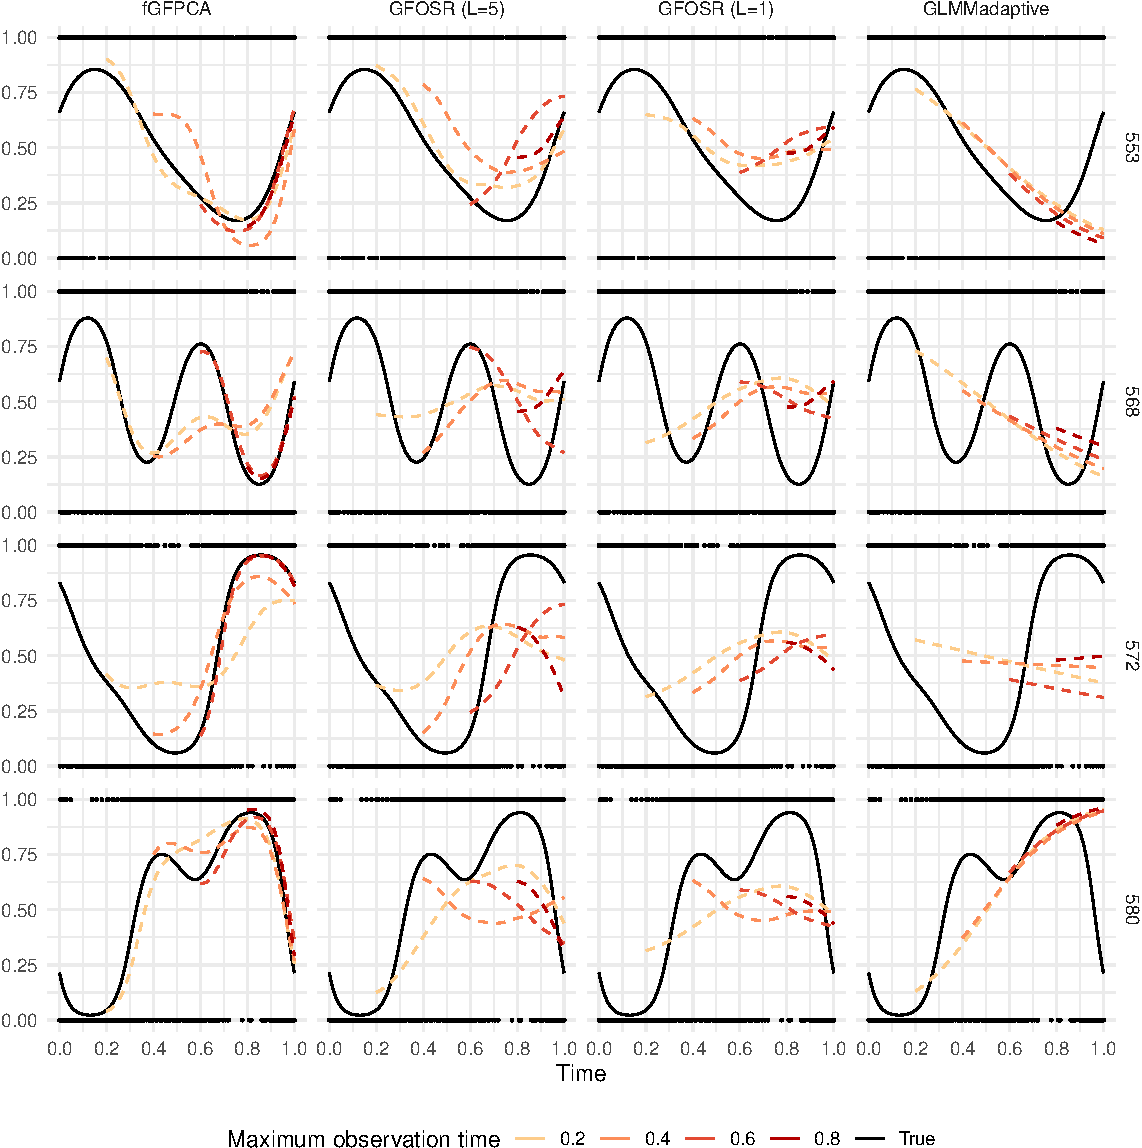
\includegraphics{manuscript_files/figure-latex/fig_large_sim-1.pdf}

\hypertarget{ise-and-auc}{%
\subsection{ISE and AUC}\label{ise-and-auc}}

\begin{Shaded}
\begin{Highlighting}[]
\DocumentationTok{\#\# ISE container }
\NormalTok{ise\_fgfpca }\OtherTok{\textless{}{-}}\NormalTok{ ise\_adglmm }\OtherTok{\textless{}{-}}\NormalTok{ ise\_gfosr\_l1 }\OtherTok{\textless{}{-}}\NormalTok{ ise\_gfosr\_l5 }\OtherTok{\textless{}{-}} 
  \FunctionTok{array}\NormalTok{(}\ConstantTok{NA}\NormalTok{, }\AttributeTok{dim =} \FunctionTok{c}\NormalTok{(}\FunctionTok{length}\NormalTok{(window)}\SpecialCharTok{{-}}\DecValTok{2}\NormalTok{, }\FunctionTok{length}\NormalTok{(window)}\SpecialCharTok{{-}}\DecValTok{2}\NormalTok{, M))}
\CommentTok{\# dims: prediction window, max obs time, simulation iter}
\end{Highlighting}
\end{Shaded}

\begin{Shaded}
\begin{Highlighting}[]
\DocumentationTok{\#\# calculation}
\ControlFlowTok{for}\NormalTok{(m }\ControlFlowTok{in} \DecValTok{1}\SpecialCharTok{:}\NormalTok{M)\{}
  \CommentTok{\# this\_df \textless{}{-} pred\_list\_all[[m]]}
\NormalTok{  ise\_tb }\OtherTok{\textless{}{-}}\NormalTok{ pred\_list\_all[[m]] }\SpecialCharTok{\%\textgreater{}\%}
    \FunctionTok{mutate}\NormalTok{(}\AttributeTok{err1 =}\NormalTok{ (pred0}\FloatTok{.2}\SpecialCharTok{{-}}\NormalTok{eta\_i)}\SpecialCharTok{\^{}}\DecValTok{2}\NormalTok{,}
           \AttributeTok{err2 =}\NormalTok{ (pred0}\FloatTok{.4}\SpecialCharTok{{-}}\NormalTok{eta\_i)}\SpecialCharTok{\^{}}\DecValTok{2}\NormalTok{,}
           \AttributeTok{err3 =}\NormalTok{ (pred0}\FloatTok{.6}\SpecialCharTok{{-}}\NormalTok{eta\_i)}\SpecialCharTok{\^{}}\DecValTok{2}\NormalTok{,}
           \AttributeTok{err4 =}\NormalTok{ (pred0}\FloatTok{.8}\SpecialCharTok{{-}}\NormalTok{eta\_i)}\SpecialCharTok{\^{}}\DecValTok{2}\NormalTok{) }\SpecialCharTok{\%\textgreater{}\%}
    \FunctionTok{select}\NormalTok{(id, t, }\FunctionTok{starts\_with}\NormalTok{(}\StringTok{"err"}\NormalTok{)) }\SpecialCharTok{\%\textgreater{}\%} 
    \FunctionTok{mutate}\NormalTok{(}\AttributeTok{window =} \FunctionTok{cut}\NormalTok{(t, }\AttributeTok{breaks =}\NormalTok{ window, }\AttributeTok{include.lowest =}\NormalTok{ T)) }\SpecialCharTok{\%\textgreater{}\%} 
    \FunctionTok{group\_by}\NormalTok{(window, id) }\SpecialCharTok{\%\textgreater{}\%} 
    \FunctionTok{summarise\_at}\NormalTok{(}\FunctionTok{vars}\NormalTok{(err1, err2, err3, err4), sum) }\SpecialCharTok{\%\textgreater{}\%} 
    \FunctionTok{group\_by}\NormalTok{(window) }\SpecialCharTok{\%\textgreater{}\%} 
    \FunctionTok{summarize\_at}\NormalTok{(}\FunctionTok{vars}\NormalTok{(err1, err2, err3, err4), mean) }\SpecialCharTok{\%\textgreater{}\%}
    \FunctionTok{filter}\NormalTok{(window }\SpecialCharTok{!=} \StringTok{"[0,0.2]"}\NormalTok{) }\SpecialCharTok{\%\textgreater{}\%} 
    \FunctionTok{select}\NormalTok{(}\FunctionTok{starts\_with}\NormalTok{(}\StringTok{"err"}\NormalTok{))}
\NormalTok{  ise\_fgfpca[, ,m] }\OtherTok{\textless{}{-}} \FunctionTok{as.matrix}\NormalTok{(ise\_tb)}
  
  
\NormalTok{\}}

\NormalTok{mean\_ise\_fgfpca }\OtherTok{\textless{}{-}} \FunctionTok{apply}\NormalTok{(ise\_fgfpca, }\FunctionTok{c}\NormalTok{(}\DecValTok{1}\NormalTok{, }\DecValTok{2}\NormalTok{), mean)}

\CommentTok{\# mean\_ise \textless{}{-} data.frame(mean\_ise) \%\textgreater{}\%}
\CommentTok{\#   mutate(Window = c("(0.2, 0.4]", "(0.4, 0.6]", "(0.6, 0.8]", "(0.8, 1.0]"),}
\CommentTok{\#          .before = 1)}
\FunctionTok{colnames}\NormalTok{(mean\_ise\_fgfpca) }\OtherTok{\textless{}{-}} \FunctionTok{c}\NormalTok{(}\StringTok{"0.2"}\NormalTok{, }\StringTok{"0.4"}\NormalTok{, }\StringTok{"0.6"}\NormalTok{, }\StringTok{"0.8"}\NormalTok{)}
\end{Highlighting}
\end{Shaded}

\begin{Shaded}
\begin{Highlighting}[]
\DocumentationTok{\#\# calculation}
\ControlFlowTok{for}\NormalTok{(m }\ControlFlowTok{in} \DecValTok{1}\SpecialCharTok{:}\NormalTok{M)\{}
  \CommentTok{\# this\_df \textless{}{-} pred\_list\_gfosr\_l1[[m]]}
\NormalTok{  ise\_tb }\OtherTok{\textless{}{-}}\NormalTok{ pred\_list\_ref[[m]] }\SpecialCharTok{\%\textgreater{}\%}
    \FunctionTok{mutate}\NormalTok{(}\AttributeTok{err1 =}\NormalTok{ (pred0}\FloatTok{.2}\SpecialCharTok{{-}}\NormalTok{eta\_i)}\SpecialCharTok{\^{}}\DecValTok{2}\NormalTok{,}
           \AttributeTok{err2 =}\NormalTok{ (pred0}\FloatTok{.4}\SpecialCharTok{{-}}\NormalTok{eta\_i)}\SpecialCharTok{\^{}}\DecValTok{2}\NormalTok{,}
           \AttributeTok{err3 =}\NormalTok{ (pred0}\FloatTok{.6}\SpecialCharTok{{-}}\NormalTok{eta\_i)}\SpecialCharTok{\^{}}\DecValTok{2}\NormalTok{,}
           \AttributeTok{err4 =}\NormalTok{ (pred0}\FloatTok{.8}\SpecialCharTok{{-}}\NormalTok{eta\_i)}\SpecialCharTok{\^{}}\DecValTok{2}\NormalTok{) }\SpecialCharTok{\%\textgreater{}\%}
    \FunctionTok{select}\NormalTok{(id, t, }\FunctionTok{starts\_with}\NormalTok{(}\StringTok{"err"}\NormalTok{)) }\SpecialCharTok{\%\textgreater{}\%} 
    \FunctionTok{mutate}\NormalTok{(}\AttributeTok{window =} \FunctionTok{cut}\NormalTok{(t, }\AttributeTok{breaks =}\NormalTok{ window, }\AttributeTok{include.lowest =}\NormalTok{ T)) }\SpecialCharTok{\%\textgreater{}\%} 
    \FunctionTok{group\_by}\NormalTok{(window, id) }\SpecialCharTok{\%\textgreater{}\%} 
    \FunctionTok{summarise\_at}\NormalTok{(}\FunctionTok{vars}\NormalTok{(err1, err2, err3, err4), sum) }\SpecialCharTok{\%\textgreater{}\%} 
    \FunctionTok{group\_by}\NormalTok{(window) }\SpecialCharTok{\%\textgreater{}\%} 
    \FunctionTok{summarize\_at}\NormalTok{(}\FunctionTok{vars}\NormalTok{(err1, err2, err3, err4), mean) }\SpecialCharTok{\%\textgreater{}\%}
    \FunctionTok{filter}\NormalTok{(window }\SpecialCharTok{!=} \StringTok{"[0,0.2]"}\NormalTok{) }\SpecialCharTok{\%\textgreater{}\%} 
    \FunctionTok{select}\NormalTok{(}\FunctionTok{starts\_with}\NormalTok{(}\StringTok{"err"}\NormalTok{))}
\NormalTok{  ise\_adglmm[, ,m] }\OtherTok{\textless{}{-}} \FunctionTok{as.matrix}\NormalTok{(ise\_tb)}
\NormalTok{\}}

\NormalTok{mean\_ise\_adglmm }\OtherTok{\textless{}{-}} \FunctionTok{apply}\NormalTok{(ise\_adglmm, }\FunctionTok{c}\NormalTok{(}\DecValTok{1}\NormalTok{, }\DecValTok{2}\NormalTok{), mean)}
\FunctionTok{colnames}\NormalTok{(mean\_ise\_adglmm) }\OtherTok{\textless{}{-}} \FunctionTok{c}\NormalTok{(}\StringTok{"0.2"}\NormalTok{, }\StringTok{"0.4"}\NormalTok{, }\StringTok{"0.6"}\NormalTok{, }\StringTok{"0.8"}\NormalTok{)}
\end{Highlighting}
\end{Shaded}

\begin{Shaded}
\begin{Highlighting}[]
\DocumentationTok{\#\# calculation}
\ControlFlowTok{for}\NormalTok{(m }\ControlFlowTok{in} \DecValTok{1}\SpecialCharTok{:}\NormalTok{M)\{}
  \CommentTok{\# this\_df \textless{}{-} pred\_list\_ref[[m]]}
\NormalTok{  ise\_tb }\OtherTok{\textless{}{-}}\NormalTok{ pred\_list\_gfosr\_l1[[m]] }\SpecialCharTok{\%\textgreater{}\%}
    \FunctionTok{mutate}\NormalTok{(}\AttributeTok{err1 =}\NormalTok{ (pred\_w1}\SpecialCharTok{{-}}\NormalTok{eta\_i)}\SpecialCharTok{\^{}}\DecValTok{2}\NormalTok{,}
           \AttributeTok{err2 =}\NormalTok{ (pred\_w2}\SpecialCharTok{{-}}\NormalTok{eta\_i)}\SpecialCharTok{\^{}}\DecValTok{2}\NormalTok{,}
           \AttributeTok{err3 =}\NormalTok{ (pred\_w3}\SpecialCharTok{{-}}\NormalTok{eta\_i)}\SpecialCharTok{\^{}}\DecValTok{2}\NormalTok{,}
           \AttributeTok{err4 =}\NormalTok{ (pred\_w4}\SpecialCharTok{{-}}\NormalTok{eta\_i)}\SpecialCharTok{\^{}}\DecValTok{2}\NormalTok{) }\SpecialCharTok{\%\textgreater{}\%}
    \FunctionTok{select}\NormalTok{(id, t, }\FunctionTok{starts\_with}\NormalTok{(}\StringTok{"err"}\NormalTok{), window) }\SpecialCharTok{\%\textgreater{}\%} 
    \CommentTok{\# mutate(window = factor(window, levels = 1:5, }
    \CommentTok{\#                        labels = c("[0,0.2]", "(0.2,0.4]", "(0.4,0.6]",))) \%\textgreater{}\% }
    \FunctionTok{group\_by}\NormalTok{(window, id) }\SpecialCharTok{\%\textgreater{}\%} 
    \FunctionTok{summarise\_at}\NormalTok{(}\FunctionTok{vars}\NormalTok{(err1, err2, err3, err4), sum) }\SpecialCharTok{\%\textgreater{}\%} 
    \FunctionTok{group\_by}\NormalTok{(window) }\SpecialCharTok{\%\textgreater{}\%} 
    \FunctionTok{summarize\_at}\NormalTok{(}\FunctionTok{vars}\NormalTok{(err1, err2, err3, err4), mean) }\SpecialCharTok{\%\textgreater{}\%}
    \FunctionTok{filter}\NormalTok{(window }\SpecialCharTok{!=} \DecValTok{1}\NormalTok{) }\SpecialCharTok{\%\textgreater{}\%} 
    \FunctionTok{select}\NormalTok{(}\FunctionTok{starts\_with}\NormalTok{(}\StringTok{"err"}\NormalTok{))}
\NormalTok{  ise\_gfosr\_l1[, ,m] }\OtherTok{\textless{}{-}} \FunctionTok{as.matrix}\NormalTok{(ise\_tb)}
\NormalTok{\}}

\NormalTok{mean\_ise\_gfosr\_l1 }\OtherTok{\textless{}{-}} \FunctionTok{apply}\NormalTok{(ise\_gfosr\_l1, }\FunctionTok{c}\NormalTok{(}\DecValTok{1}\NormalTok{, }\DecValTok{2}\NormalTok{), mean)}
\FunctionTok{colnames}\NormalTok{(mean\_ise\_gfosr\_l1) }\OtherTok{\textless{}{-}} \FunctionTok{c}\NormalTok{(}\StringTok{"0.2"}\NormalTok{, }\StringTok{"0.4"}\NormalTok{, }\StringTok{"0.6"}\NormalTok{, }\StringTok{"0.8"}\NormalTok{)}
\end{Highlighting}
\end{Shaded}

\begin{Shaded}
\begin{Highlighting}[]
\DocumentationTok{\#\# calculation}
\ControlFlowTok{for}\NormalTok{(m }\ControlFlowTok{in} \DecValTok{1}\SpecialCharTok{:}\NormalTok{M)\{}
  \CommentTok{\# this\_df \textless{}{-} pred\_list\_ref[[m]]}
\NormalTok{  ise\_tb }\OtherTok{\textless{}{-}}\NormalTok{ pred\_list\_gfosr\_l5[[m]] }\SpecialCharTok{\%\textgreater{}\%}
    \FunctionTok{mutate}\NormalTok{(}\AttributeTok{err1 =}\NormalTok{ (pred\_w1}\SpecialCharTok{{-}}\NormalTok{eta\_i)}\SpecialCharTok{\^{}}\DecValTok{2}\NormalTok{,}
           \AttributeTok{err2 =}\NormalTok{ (pred\_w2}\SpecialCharTok{{-}}\NormalTok{eta\_i)}\SpecialCharTok{\^{}}\DecValTok{2}\NormalTok{,}
           \AttributeTok{err3 =}\NormalTok{ (pred\_w3}\SpecialCharTok{{-}}\NormalTok{eta\_i)}\SpecialCharTok{\^{}}\DecValTok{2}\NormalTok{,}
           \AttributeTok{err4 =}\NormalTok{ (pred\_w4}\SpecialCharTok{{-}}\NormalTok{eta\_i)}\SpecialCharTok{\^{}}\DecValTok{2}\NormalTok{) }\SpecialCharTok{\%\textgreater{}\%}
    \FunctionTok{select}\NormalTok{(id, t, }\FunctionTok{starts\_with}\NormalTok{(}\StringTok{"err"}\NormalTok{), window) }\SpecialCharTok{\%\textgreater{}\%} 
    \CommentTok{\# mutate(window = factor(window, levels = 1:5, }
    \CommentTok{\#                        labels = c("[0,0.2]", "(0.2,0.4]", "(0.4,0.6]",))) \%\textgreater{}\% }
    \FunctionTok{group\_by}\NormalTok{(window, id) }\SpecialCharTok{\%\textgreater{}\%} 
    \FunctionTok{summarise\_at}\NormalTok{(}\FunctionTok{vars}\NormalTok{(err1, err2, err3, err4), sum) }\SpecialCharTok{\%\textgreater{}\%} 
    \FunctionTok{group\_by}\NormalTok{(window) }\SpecialCharTok{\%\textgreater{}\%} 
    \FunctionTok{summarize\_at}\NormalTok{(}\FunctionTok{vars}\NormalTok{(err1, err2, err3, err4), mean) }\SpecialCharTok{\%\textgreater{}\%}
    \FunctionTok{filter}\NormalTok{(window }\SpecialCharTok{!=} \DecValTok{1}\NormalTok{) }\SpecialCharTok{\%\textgreater{}\%} 
    \FunctionTok{select}\NormalTok{(}\FunctionTok{starts\_with}\NormalTok{(}\StringTok{"err"}\NormalTok{))}
\NormalTok{  ise\_gfosr\_l5[, ,m] }\OtherTok{\textless{}{-}} \FunctionTok{as.matrix}\NormalTok{(ise\_tb)}
\NormalTok{\}}

\NormalTok{mean\_ise\_gfosr\_l5 }\OtherTok{\textless{}{-}} \FunctionTok{apply}\NormalTok{(ise\_gfosr\_l5, }\FunctionTok{c}\NormalTok{(}\DecValTok{1}\NormalTok{, }\DecValTok{2}\NormalTok{), mean)}
\FunctionTok{colnames}\NormalTok{(mean\_ise\_gfosr\_l5) }\OtherTok{\textless{}{-}} \FunctionTok{c}\NormalTok{(}\StringTok{"0.2"}\NormalTok{, }\StringTok{"0.4"}\NormalTok{, }\StringTok{"0.6"}\NormalTok{, }\StringTok{"0.8"}\NormalTok{)}
\end{Highlighting}
\end{Shaded}

\begin{Shaded}
\begin{Highlighting}[]
\DocumentationTok{\#\# a function to calculate AUC}
\NormalTok{get\_auc }\OtherTok{\textless{}{-}} \ControlFlowTok{function}\NormalTok{(y, pred)\{}
  \ControlFlowTok{if}\NormalTok{(}\FunctionTok{sum}\NormalTok{(}\FunctionTok{is.na}\NormalTok{(y))}\SpecialCharTok{\textgreater{}}\DecValTok{0} \SpecialCharTok{|} \FunctionTok{sum}\NormalTok{(}\FunctionTok{is.na}\NormalTok{(pred))}\SpecialCharTok{\textgreater{}}\DecValTok{0}\NormalTok{)\{}
\NormalTok{    auc }\OtherTok{\textless{}{-}} \ConstantTok{NA}
\NormalTok{  \}}
  \ControlFlowTok{else}\NormalTok{\{}
\NormalTok{    this\_perf }\OtherTok{\textless{}{-}} \FunctionTok{performance}\NormalTok{(}\FunctionTok{prediction}\NormalTok{(pred, y), }\AttributeTok{measure =} \StringTok{"auc"}\NormalTok{)}
\NormalTok{    auc }\OtherTok{\textless{}{-}}\NormalTok{ this\_perf}\SpecialCharTok{@}\NormalTok{y.values[[}\DecValTok{1}\NormalTok{]]}
\NormalTok{  \}}
  \FunctionTok{return}\NormalTok{(auc)}
\NormalTok{\}}
\end{Highlighting}
\end{Shaded}

\begin{Shaded}
\begin{Highlighting}[]
\DocumentationTok{\#\# auc container }
\NormalTok{auc\_fgfpca }\OtherTok{\textless{}{-}}\NormalTok{ auc\_adglmm }\OtherTok{\textless{}{-}}\NormalTok{ auc\_gfosr\_l1 }\OtherTok{\textless{}{-}}\NormalTok{ auc\_gfosr\_l5 }\OtherTok{\textless{}{-}} 
  \FunctionTok{array}\NormalTok{(}\ConstantTok{NA}\NormalTok{, }\AttributeTok{dim =} \FunctionTok{c}\NormalTok{(}\FunctionTok{length}\NormalTok{(window)}\SpecialCharTok{{-}}\DecValTok{2}\NormalTok{, }\FunctionTok{length}\NormalTok{(window)}\SpecialCharTok{{-}}\DecValTok{2}\NormalTok{, M))}
\end{Highlighting}
\end{Shaded}

\begin{Shaded}
\begin{Highlighting}[]
\ControlFlowTok{for}\NormalTok{(m }\ControlFlowTok{in} \DecValTok{1}\SpecialCharTok{:}\NormalTok{M)\{}
\NormalTok{  this\_df }\OtherTok{\textless{}{-}}\NormalTok{ pred\_list\_all[[m]]}
\NormalTok{  auc\_tb }\OtherTok{\textless{}{-}}\NormalTok{ this\_df }\SpecialCharTok{\%\textgreater{}\%} 
    \FunctionTok{mutate}\NormalTok{(}\AttributeTok{window =} \FunctionTok{cut}\NormalTok{(t, }\AttributeTok{breaks =}\NormalTok{ window, }\AttributeTok{include.lowest =}\NormalTok{ T)) }\SpecialCharTok{\%\textgreater{}\%} 
    \FunctionTok{select}\NormalTok{(Y, }\FunctionTok{starts\_with}\NormalTok{(}\StringTok{"pred"}\NormalTok{), window) }\SpecialCharTok{\%\textgreater{}\%}
    \FunctionTok{group\_by}\NormalTok{(window) }\SpecialCharTok{\%\textgreater{}\%}
    \FunctionTok{summarise}\NormalTok{(}\AttributeTok{auc1 =} \FunctionTok{get\_auc}\NormalTok{(Y, pred0}\FloatTok{.2}\NormalTok{),}
              \AttributeTok{auc2 =} \FunctionTok{get\_auc}\NormalTok{(Y, pred0}\FloatTok{.4}\NormalTok{),}
              \AttributeTok{auc3 =} \FunctionTok{get\_auc}\NormalTok{(Y, pred0}\FloatTok{.6}\NormalTok{),}
              \AttributeTok{auc4 =} \FunctionTok{get\_auc}\NormalTok{(Y, pred0}\FloatTok{.8}\NormalTok{)) }\SpecialCharTok{\%\textgreater{}\%}
    \FunctionTok{filter}\NormalTok{(window }\SpecialCharTok{!=} \StringTok{"[0,0.2]"}\NormalTok{) }\SpecialCharTok{\%\textgreater{}\%} 
    \FunctionTok{select}\NormalTok{(}\FunctionTok{starts\_with}\NormalTok{(}\StringTok{"auc"}\NormalTok{))}
\NormalTok{  auc\_fgfpca[, ,m] }\OtherTok{\textless{}{-}} \FunctionTok{as.matrix}\NormalTok{(auc\_tb)}
\NormalTok{\}}


\NormalTok{mean\_auc\_fgfpca }\OtherTok{\textless{}{-}} \FunctionTok{apply}\NormalTok{(auc\_fgfpca, }\FunctionTok{c}\NormalTok{(}\DecValTok{1}\NormalTok{, }\DecValTok{2}\NormalTok{), mean)}
\CommentTok{\# mean\_auc \textless{}{-} data.frame(mean\_auc) \%\textgreater{}\% }
\CommentTok{\#   mutate(Window = c("(0.2, 0.4]", "(0.4, 0.6]", "(0.6, 0.8]", "(0.8, 1.0]"),}
\CommentTok{\#          .before = 1)}
\FunctionTok{colnames}\NormalTok{(mean\_auc\_fgfpca) }\OtherTok{\textless{}{-}} \FunctionTok{c}\NormalTok{(}\StringTok{"0.2"}\NormalTok{, }\StringTok{"0.4"}\NormalTok{, }\StringTok{"0.6"}\NormalTok{, }\StringTok{"0.8"}\NormalTok{)}
\end{Highlighting}
\end{Shaded}

\begin{Shaded}
\begin{Highlighting}[]
\ControlFlowTok{for}\NormalTok{(m }\ControlFlowTok{in} \DecValTok{1}\SpecialCharTok{:}\NormalTok{M)\{}
\NormalTok{  this\_df }\OtherTok{\textless{}{-}}\NormalTok{ pred\_list\_ref[[m]]}
\NormalTok{  auc\_tb }\OtherTok{\textless{}{-}}\NormalTok{ this\_df }\SpecialCharTok{\%\textgreater{}\%} 
    \FunctionTok{mutate}\NormalTok{(}\AttributeTok{window =} \FunctionTok{cut}\NormalTok{(t, }\AttributeTok{breaks =}\NormalTok{ window, }\AttributeTok{include.lowest =}\NormalTok{ T)) }\SpecialCharTok{\%\textgreater{}\%} 
    \FunctionTok{select}\NormalTok{(Y, }\FunctionTok{starts\_with}\NormalTok{(}\StringTok{"pred"}\NormalTok{), window) }\SpecialCharTok{\%\textgreater{}\%}
    \FunctionTok{group\_by}\NormalTok{(window) }\SpecialCharTok{\%\textgreater{}\%}
    \FunctionTok{summarise}\NormalTok{(}\AttributeTok{auc1 =} \FunctionTok{get\_auc}\NormalTok{(Y, pred0}\FloatTok{.2}\NormalTok{),}
              \AttributeTok{auc2 =} \FunctionTok{get\_auc}\NormalTok{(Y, pred0}\FloatTok{.4}\NormalTok{),}
              \AttributeTok{auc3 =} \FunctionTok{get\_auc}\NormalTok{(Y, pred0}\FloatTok{.6}\NormalTok{),}
              \AttributeTok{auc4 =} \FunctionTok{get\_auc}\NormalTok{(Y, pred0}\FloatTok{.8}\NormalTok{)) }\SpecialCharTok{\%\textgreater{}\%}
    \FunctionTok{filter}\NormalTok{(window }\SpecialCharTok{!=} \StringTok{"[0,0.2]"}\NormalTok{) }\SpecialCharTok{\%\textgreater{}\%} 
    \FunctionTok{select}\NormalTok{(}\FunctionTok{starts\_with}\NormalTok{(}\StringTok{"auc"}\NormalTok{))}
\NormalTok{  auc\_adglmm[, ,m] }\OtherTok{\textless{}{-}} \FunctionTok{as.matrix}\NormalTok{(auc\_tb)}

\NormalTok{\}}


\NormalTok{mean\_auc\_adglmm }\OtherTok{\textless{}{-}} \FunctionTok{apply}\NormalTok{(auc\_adglmm, }\FunctionTok{c}\NormalTok{(}\DecValTok{1}\NormalTok{, }\DecValTok{2}\NormalTok{), mean)}
\FunctionTok{colnames}\NormalTok{(mean\_auc\_adglmm) }\OtherTok{\textless{}{-}} \FunctionTok{c}\NormalTok{(}\StringTok{"0.2"}\NormalTok{, }\StringTok{"0.4"}\NormalTok{, }\StringTok{"0.6"}\NormalTok{, }\StringTok{"0.8"}\NormalTok{)}
\end{Highlighting}
\end{Shaded}

\begin{Shaded}
\begin{Highlighting}[]
\ControlFlowTok{for}\NormalTok{(m }\ControlFlowTok{in} \DecValTok{1}\SpecialCharTok{:}\NormalTok{M)\{}
\NormalTok{  this\_df }\OtherTok{\textless{}{-}}\NormalTok{ pred\_list\_gfosr\_l1[[m]]}
\NormalTok{  auc\_tb }\OtherTok{\textless{}{-}}\NormalTok{ this\_df }\SpecialCharTok{\%\textgreater{}\%} 
    \FunctionTok{select}\NormalTok{(Y, }\FunctionTok{starts\_with}\NormalTok{(}\StringTok{"pred"}\NormalTok{), window) }\SpecialCharTok{\%\textgreater{}\%}
    \FunctionTok{group\_by}\NormalTok{(window) }\SpecialCharTok{\%\textgreater{}\%}
    \FunctionTok{summarise}\NormalTok{(}\AttributeTok{auc1 =} \FunctionTok{get\_auc}\NormalTok{(Y, pred\_w1),}
              \AttributeTok{auc2 =} \FunctionTok{get\_auc}\NormalTok{(Y, pred\_w2),}
              \AttributeTok{auc3 =} \FunctionTok{get\_auc}\NormalTok{(Y, pred\_w3),}
              \AttributeTok{auc4 =} \FunctionTok{get\_auc}\NormalTok{(Y, pred\_w4)) }\SpecialCharTok{\%\textgreater{}\%}
    \FunctionTok{filter}\NormalTok{(window }\SpecialCharTok{!=} \DecValTok{1}\NormalTok{) }\SpecialCharTok{\%\textgreater{}\%} 
    \FunctionTok{select}\NormalTok{(}\FunctionTok{starts\_with}\NormalTok{(}\StringTok{"auc"}\NormalTok{))}
\NormalTok{  auc\_gfosr\_l1[, ,m] }\OtherTok{\textless{}{-}} \FunctionTok{as.matrix}\NormalTok{(auc\_tb)}

\NormalTok{\}}


\NormalTok{mean\_auc\_gfosr\_l1 }\OtherTok{\textless{}{-}} \FunctionTok{apply}\NormalTok{(auc\_gfosr\_l1, }\FunctionTok{c}\NormalTok{(}\DecValTok{1}\NormalTok{, }\DecValTok{2}\NormalTok{), mean)}
\FunctionTok{colnames}\NormalTok{(mean\_auc\_gfosr\_l1) }\OtherTok{\textless{}{-}} \FunctionTok{c}\NormalTok{(}\StringTok{"0.2"}\NormalTok{, }\StringTok{"0.4"}\NormalTok{, }\StringTok{"0.6"}\NormalTok{, }\StringTok{"0.8"}\NormalTok{)}
\end{Highlighting}
\end{Shaded}

\begin{Shaded}
\begin{Highlighting}[]
\ControlFlowTok{for}\NormalTok{(m }\ControlFlowTok{in} \DecValTok{1}\SpecialCharTok{:}\NormalTok{M)\{}
\NormalTok{  this\_df }\OtherTok{\textless{}{-}}\NormalTok{ pred\_list\_gfosr\_l5[[m]]}
\NormalTok{  auc\_tb }\OtherTok{\textless{}{-}}\NormalTok{ this\_df }\SpecialCharTok{\%\textgreater{}\%} 
    \FunctionTok{select}\NormalTok{(Y, }\FunctionTok{starts\_with}\NormalTok{(}\StringTok{"pred"}\NormalTok{), window) }\SpecialCharTok{\%\textgreater{}\%}
    \FunctionTok{group\_by}\NormalTok{(window) }\SpecialCharTok{\%\textgreater{}\%}
    \FunctionTok{summarise}\NormalTok{(}\AttributeTok{auc1 =} \FunctionTok{get\_auc}\NormalTok{(Y, pred\_w1),}
              \AttributeTok{auc2 =} \FunctionTok{get\_auc}\NormalTok{(Y, pred\_w2),}
              \AttributeTok{auc3 =} \FunctionTok{get\_auc}\NormalTok{(Y, pred\_w3),}
              \AttributeTok{auc4 =} \FunctionTok{get\_auc}\NormalTok{(Y, pred\_w4)) }\SpecialCharTok{\%\textgreater{}\%}
    \FunctionTok{filter}\NormalTok{(window }\SpecialCharTok{!=} \DecValTok{1}\NormalTok{) }\SpecialCharTok{\%\textgreater{}\%} 
    \FunctionTok{select}\NormalTok{(}\FunctionTok{starts\_with}\NormalTok{(}\StringTok{"auc"}\NormalTok{))}
\NormalTok{  auc\_gfosr\_l5[, ,m] }\OtherTok{\textless{}{-}} \FunctionTok{as.matrix}\NormalTok{(auc\_tb)}

\NormalTok{\}}


\NormalTok{mean\_auc\_gfosr\_l5 }\OtherTok{\textless{}{-}} \FunctionTok{apply}\NormalTok{(auc\_gfosr\_l5, }\FunctionTok{c}\NormalTok{(}\DecValTok{1}\NormalTok{, }\DecValTok{2}\NormalTok{), mean)}
\FunctionTok{colnames}\NormalTok{(mean\_auc\_gfosr\_l5) }\OtherTok{\textless{}{-}} \FunctionTok{c}\NormalTok{(}\StringTok{"0.2"}\NormalTok{, }\StringTok{"0.4"}\NormalTok{, }\StringTok{"0.6"}\NormalTok{, }\StringTok{"0.8"}\NormalTok{)}
\end{Highlighting}
\end{Shaded}

\begin{Shaded}
\begin{Highlighting}[]
\NormalTok{fgfpca1 }\OtherTok{\textless{}{-}} \FunctionTok{rbind}\NormalTok{(mean\_ise\_fgfpca ,mean\_auc\_fgfpca) }\SpecialCharTok{\%\textgreater{}\%} \FunctionTok{as\_tibble}\NormalTok{() }\SpecialCharTok{\%\textgreater{}\%}
  \FunctionTok{mutate}\NormalTok{(}\AttributeTok{Window =} \FunctionTok{rep}\NormalTok{(}\FunctionTok{c}\NormalTok{(}\StringTok{"(0.2, 0.4]"}\NormalTok{, }\StringTok{"(0.4, 0.6]"}\NormalTok{, }\StringTok{"(0.6, 0.8]"}\NormalTok{, }\StringTok{"(0.8, 1.0]"}\NormalTok{), }\DecValTok{2}\NormalTok{), }\AttributeTok{.before=}\DecValTok{1}\NormalTok{)}
\NormalTok{gfosr\_l5\_1 }\OtherTok{\textless{}{-}} \FunctionTok{rbind}\NormalTok{(mean\_ise\_gfosr\_l5 ,mean\_auc\_gfosr\_l5) }\SpecialCharTok{\%\textgreater{}\%} \FunctionTok{as\_tibble}\NormalTok{()}
\NormalTok{gfosr\_l1\_1 }\OtherTok{\textless{}{-}} \FunctionTok{rbind}\NormalTok{(mean\_ise\_gfosr\_l1 ,mean\_auc\_gfosr\_l1) }\SpecialCharTok{\%\textgreater{}\%} \FunctionTok{as\_tibble}\NormalTok{()}
\NormalTok{adglmm1 }\OtherTok{\textless{}{-}} \FunctionTok{rbind}\NormalTok{(mean\_ise\_adglmm ,mean\_auc\_adglmm) }\SpecialCharTok{\%\textgreater{}\%} \FunctionTok{as\_tibble}\NormalTok{() }

\FunctionTok{bind\_cols}\NormalTok{(fgfpca1, gfosr\_l5\_1, gfosr\_l1\_1, adglmm1, }\AttributeTok{.name\_repair =} \StringTok{"minimal"}\NormalTok{) }\SpecialCharTok{\%\textgreater{}\%}
  \FunctionTok{kable}\NormalTok{(}\AttributeTok{digits =} \DecValTok{3}\NormalTok{, }\AttributeTok{booktabs=}\NormalTok{T,}
        \AttributeTok{table.attr=}\StringTok{"style=}\SpecialCharTok{\textbackslash{}"}\StringTok{color:black;}\SpecialCharTok{\textbackslash{}"}\StringTok{"}\NormalTok{) }\SpecialCharTok{\%\textgreater{}\%}
  \FunctionTok{kable\_styling}\NormalTok{(}\AttributeTok{full\_width =}\NormalTok{ F) }\SpecialCharTok{\%\textgreater{}\%} 
  \FunctionTok{add\_header\_above}\NormalTok{(}\FunctionTok{c}\NormalTok{(}\StringTok{" "} \OtherTok{=} \DecValTok{1}\NormalTok{, }\StringTok{"fGFPCA"} \OtherTok{=} \DecValTok{4}\NormalTok{, }\StringTok{"GFOSR (L=5)"} \OtherTok{=} \DecValTok{4}\NormalTok{, }
                     \StringTok{"GFOSR (L=1)"} \OtherTok{=} \DecValTok{4}\NormalTok{, }\StringTok{"GLMMadaptive"} \OtherTok{=} \DecValTok{4}\NormalTok{)) }\SpecialCharTok{\%\textgreater{}\%}
  \FunctionTok{add\_header\_above}\NormalTok{(}\FunctionTok{c}\NormalTok{(}\StringTok{" "} \OtherTok{=} \DecValTok{1}\NormalTok{, }\StringTok{"Maximum observation time"} \OtherTok{=} \DecValTok{16}\NormalTok{)) }\SpecialCharTok{\%\textgreater{}\%}
  \FunctionTok{group\_rows}\NormalTok{(}\AttributeTok{index =} \FunctionTok{c}\NormalTok{(}\StringTok{"ISE"}\OtherTok{=} \DecValTok{4}\NormalTok{, }\StringTok{"AUC"} \OtherTok{=} \DecValTok{4}\NormalTok{)) }\SpecialCharTok{\%\textgreater{}\%}
  \FunctionTok{landscape}\NormalTok{()}
\end{Highlighting}
\end{Shaded}

\begin{landscape}\begin{table}
\centering
\begin{tabular}{lrrrrrrrrrrrrrrrr}
\toprule
\multicolumn{1}{c}{ } & \multicolumn{16}{c}{Maximum observation time} \\
\cmidrule(l{3pt}r{3pt}){2-17}
\multicolumn{1}{c}{ } & \multicolumn{4}{c}{fGFPCA} & \multicolumn{4}{c}{GFOSR (L=5)} & \multicolumn{4}{c}{GFOSR (L=1)} & \multicolumn{4}{c}{GLMMadaptive} \\
\cmidrule(l{3pt}r{3pt}){2-5} \cmidrule(l{3pt}r{3pt}){6-9} \cmidrule(l{3pt}r{3pt}){10-13} \cmidrule(l{3pt}r{3pt}){14-17}
Window & 0.2 & 0.4 & 0.6 & 0.8 & 0.2 & 0.4 & 0.6 & 0.8 & 0.2 & 0.4 & 0.6 & 0.8 & 0.2 & 0.4 & 0.6 & 0.8\\
\midrule
\addlinespace[0.3em]
\multicolumn{17}{l}{\textbf{ISE}}\\
\hspace{1em}(0.2, 0.4] & 146.407 &  &  &  & 274.947 &  &  &  & 362.476 &  &  &  & 387.708 &  &  & \\
\hspace{1em}(0.4, 0.6] & 183.967 & 74.977 &  &  & 277.438 & 220.209 &  &  & 286.614 & 262.552 &  &  & 291.579 & 269.799 &  & \\
\hspace{1em}(0.6, 0.8] & 218.265 & 49.275 & 15.776 &  & 322.338 & 373.108 & 325.017 &  & 385.701 & 410.508 & 389.305 &  & 315.778 & 282.736 & 278.242 & \\
\hspace{1em}(0.8, 1.0] & 108.918 & 77.981 & 17.747 & 12.005 & 290.982 & 318.079 & 350.850 & 333.580 & 328.482 & 341.274 & 354.211 & 347.067 & 563.011 & 477.485 & 597.746 & 600.340\\
\addlinespace[0.3em]
\multicolumn{17}{l}{\textbf{AUC}}\\
\hspace{1em}(0.2, 0.4] & 0.748 &  &  &  & 0.686 &  &  &  & 0.624 &  &  &  & 0.591 &  &  & \\
\hspace{1em}(0.4, 0.6] & 0.664 & 0.734 &  &  & 0.563 & 0.630 &  &  & 0.543 & 0.590 &  &  & 0.524 & 0.596 &  & \\
\hspace{1em}(0.6, 0.8] & 0.715 & 0.790 & 0.803 &  & 0.669 & 0.628 & 0.676 &  & 0.604 & 0.577 & 0.615 &  & 0.669 & 0.694 & 0.687 & \\
\hspace{1em}(0.8, 1.0] & 0.740 & 0.755 & 0.781 & 0.784 & 0.626 & 0.606 & 0.552 & 0.584 & 0.588 & 0.564 & 0.537 & 0.551 & 0.514 & 0.556 & 0.526 & 0.564\\
\bottomrule
\end{tabular}
\end{table}
\end{landscape}

\hypertarget{time-minutes}{%
\subsection{Time (minutes)}\label{time-minutes}}

I chose not to report fitting and prediction time separately because it
is too difficult to tell them apart for the GFOSR models.

\begin{Shaded}
\begin{Highlighting}[]
\FunctionTok{data.frame}\NormalTok{(}
  \StringTok{"Method"} \OtherTok{=} \FunctionTok{c}\NormalTok{(}\StringTok{"fGFPCA"}\NormalTok{, }\StringTok{"GLMMadaptive"}\NormalTok{, }\StringTok{"GFOSR (L=1)"}\NormalTok{, }\StringTok{"GFOSR (L=5)"}\NormalTok{),}
  \StringTok{"Time"} \OtherTok{=} \FunctionTok{c}\NormalTok{(}\FunctionTok{mean}\NormalTok{(fit\_time}\SpecialCharTok{/}\DecValTok{60}\SpecialCharTok{+}\NormalTok{pred\_time),}
             \FunctionTok{mean}\NormalTok{(fit\_time\_ref}\SpecialCharTok{+}\NormalTok{pred\_time\_ref}\SpecialCharTok{/}\DecValTok{60}\NormalTok{),}
             \FunctionTok{mean}\NormalTok{(t\_vec\_gfosr\_l1}\SpecialCharTok{/}\DecValTok{60}\NormalTok{), }
             \FunctionTok{mean}\NormalTok{(t\_vec\_gfosr\_l5}\SpecialCharTok{/}\DecValTok{60}\NormalTok{))) }\SpecialCharTok{\%\textgreater{}\%}
  \FunctionTok{kable}\NormalTok{(}\AttributeTok{digits =} \DecValTok{3}\NormalTok{, }\AttributeTok{booktabs =}\NormalTok{ T, }\AttributeTok{table.attr =} \StringTok{"style = }\SpecialCharTok{\textbackslash{}"}\StringTok{color:black;}\SpecialCharTok{\textbackslash{}"}\StringTok{"}\NormalTok{) }\SpecialCharTok{\%\textgreater{}\%}
  \FunctionTok{kable\_styling}\NormalTok{(}\AttributeTok{full\_width =}\NormalTok{ F) }
\end{Highlighting}
\end{Shaded}

\begin{table}
\centering
\begin{tabular}{lr}
\toprule
Method & Time\\
\midrule
fGFPCA & 2.317\\
GLMMadaptive & 2.304\\
GFOSR (L=1) & 0.025\\
GFOSR (L=5) & 0.144\\
\bottomrule
\end{tabular}
\end{table}

\hypertarget{small-scale-simulation}{%
\section{Small-scale simulation}\label{small-scale-simulation}}

I have used 100 subjects for training and testing, and repeated 500
times. When fitting GLMMadpative, I reduce the number of measurements in
the training dataset to 1/10 by taking one every 10 observations. The
prediction is on the original grid.

\begin{Shaded}
\begin{Highlighting}[]
\FunctionTok{load}\NormalTok{(}\FunctionTok{here}\NormalTok{(}\StringTok{"Data/SubSimOutput\_GLMMadaptive.RData"}\NormalTok{))}

\FunctionTok{load}\NormalTok{(}\FunctionTok{here}\NormalTok{(}\StringTok{"Data/SubSimOutput\_fGFPCA.RData"}\NormalTok{))}
\NormalTok{pred\_subset\_adglmm }\OtherTok{\textless{}{-}}\NormalTok{ pred\_subset\_adglmm[}\SpecialCharTok{!}\NormalTok{num\_probs]}
\NormalTok{fit\_time\_subset\_adglmm }\OtherTok{\textless{}{-}}\NormalTok{ fit\_time\_subset\_adglmm[}\SpecialCharTok{!}\NormalTok{num\_probs]}
\NormalTok{pred\_time\_subset\_adglmm }\OtherTok{\textless{}{-}}\NormalTok{ pred\_time\_subset\_adglmm[}\SpecialCharTok{!}\NormalTok{num\_probs]}

\FunctionTok{load}\NormalTok{(}\FunctionTok{here}\NormalTok{(}\StringTok{"Data/SubSimOutput\_GFOSR\_L1.RData"}\NormalTok{))}
\NormalTok{pred\_subset\_gfosr\_l1 }\OtherTok{\textless{}{-}}\NormalTok{ pred\_list\_gfofr\_subset}
\NormalTok{t\_subset\_gfosr\_l1 }\OtherTok{\textless{}{-}}\NormalTok{ t\_vec\_gfofr\_subset}
\FunctionTok{rm}\NormalTok{(pred\_list\_gfofr\_subset, t\_vec\_gfofr\_subset)}

\FunctionTok{load}\NormalTok{(}\FunctionTok{here}\NormalTok{(}\StringTok{"Data/SubSimOutput\_GFOSR\_L5.RData"}\NormalTok{))}
\NormalTok{pred\_subset\_gfosr\_l5 }\OtherTok{\textless{}{-}}\NormalTok{ pred\_list\_gfofr\_subset}
\NormalTok{t\_subset\_gfosr\_l5 }\OtherTok{\textless{}{-}}\NormalTok{ t\_vec\_gfofr\_subset}
\FunctionTok{rm}\NormalTok{(pred\_list\_gfofr\_subset, t\_vec\_gfofr\_subset)}

\NormalTok{rand\_id }\OtherTok{\textless{}{-}} \FunctionTok{sample}\NormalTok{(}\DecValTok{101}\SpecialCharTok{:}\DecValTok{200}\NormalTok{, }\AttributeTok{size =} \DecValTok{4}\NormalTok{)}
\end{Highlighting}
\end{Shaded}

\hypertarget{figure}{%
\subsection{Figure}\label{figure}}

\begin{Shaded}
\begin{Highlighting}[]
\FunctionTok{bind\_rows}\NormalTok{(}
\NormalTok{  pred\_subset\_fGFPCA[[}\DecValTok{1}\NormalTok{]] }\SpecialCharTok{\%\textgreater{}\%} \FunctionTok{filter}\NormalTok{(id }\SpecialCharTok{\%in\%}\NormalTok{ rand\_id) }\SpecialCharTok{\%\textgreater{}\%} \FunctionTok{mutate}\NormalTok{(}\AttributeTok{method=}\StringTok{"fGFPCA"}\NormalTok{),}
\NormalTok{  pred\_subset\_gfosr\_l5[[}\DecValTok{1}\NormalTok{]] }\SpecialCharTok{\%\textgreater{}\%} \FunctionTok{filter}\NormalTok{(id }\SpecialCharTok{\%in\%}\NormalTok{ rand\_id) }\SpecialCharTok{\%\textgreater{}\%} \FunctionTok{mutate}\NormalTok{(}\AttributeTok{method =} \StringTok{"GFOSR (L=5)"}\NormalTok{) }\SpecialCharTok{\%\textgreater{}\%} 
    \FunctionTok{rename}\NormalTok{(}\AttributeTok{pred0.2=}\NormalTok{pred\_w1, }\AttributeTok{pred0.4=}\NormalTok{pred\_w2, }\AttributeTok{pred0.6=}\NormalTok{pred\_w3, }\AttributeTok{pred0.8=}\NormalTok{pred\_w4),}
\NormalTok{  pred\_subset\_gfosr\_l1[[}\DecValTok{1}\NormalTok{]] }\SpecialCharTok{\%\textgreater{}\%} \FunctionTok{filter}\NormalTok{(id }\SpecialCharTok{\%in\%}\NormalTok{ rand\_id) }\SpecialCharTok{\%\textgreater{}\%} \FunctionTok{mutate}\NormalTok{(}\AttributeTok{method =} \StringTok{"GFOSR (L=1)"}\NormalTok{) }\SpecialCharTok{\%\textgreater{}\%}
    \FunctionTok{rename}\NormalTok{(}\AttributeTok{pred0.2=}\NormalTok{pred\_w1, }\AttributeTok{pred0.4=}\NormalTok{pred\_w2, }\AttributeTok{pred0.6=}\NormalTok{pred\_w3, }\AttributeTok{pred0.8=}\NormalTok{pred\_w4),}
\NormalTok{  pred\_subset\_adglmm[[}\DecValTok{1}\NormalTok{]] }\SpecialCharTok{\%\textgreater{}\%} \FunctionTok{filter}\NormalTok{(id }\SpecialCharTok{\%in\%}\NormalTok{ rand\_id) }\SpecialCharTok{\%\textgreater{}\%} \FunctionTok{mutate}\NormalTok{(}\AttributeTok{method =} \StringTok{"GLMMadaptive"}\NormalTok{)) }\SpecialCharTok{\%\textgreater{}\%}
  \FunctionTok{mutate\_at}\NormalTok{(}\FunctionTok{vars}\NormalTok{(eta\_i, pred0}\FloatTok{.2}\NormalTok{, pred0}\FloatTok{.4}\NormalTok{, pred0}\FloatTok{.6}\NormalTok{, pred0}\FloatTok{.8}\NormalTok{), }
                \AttributeTok{.funs =} \ControlFlowTok{function}\NormalTok{(x)\{}\FunctionTok{exp}\NormalTok{(x)}\SpecialCharTok{/}\NormalTok{(}\DecValTok{1}\SpecialCharTok{+}\FunctionTok{exp}\NormalTok{(x))\}) }\SpecialCharTok{\%\textgreater{}\%}
  \FunctionTok{mutate}\NormalTok{(}\AttributeTok{method=}\FunctionTok{factor}\NormalTok{(method, }
         \AttributeTok{levels =} \FunctionTok{c}\NormalTok{(}\StringTok{"fGFPCA"}\NormalTok{, }\StringTok{"GFOSR (L=5)"}\NormalTok{, }\StringTok{"GFOSR (L=1)"}\NormalTok{,}\StringTok{"GLMMadaptive"}\NormalTok{))) }\SpecialCharTok{\%\textgreater{}\%}
  \FunctionTok{ggplot}\NormalTok{()}\SpecialCharTok{+}
  \FunctionTok{geom\_point}\NormalTok{(}\FunctionTok{aes}\NormalTok{(}\AttributeTok{x=}\NormalTok{t, }\AttributeTok{y=}\NormalTok{Y), }\AttributeTok{size =} \FloatTok{0.2}\NormalTok{)}\SpecialCharTok{+}
  \FunctionTok{geom\_line}\NormalTok{(}\FunctionTok{aes}\NormalTok{(}\AttributeTok{x=}\NormalTok{t, }\AttributeTok{y=}\NormalTok{eta\_i, }\AttributeTok{col =} \StringTok{"True"}\NormalTok{), }\AttributeTok{linetype =} \StringTok{"dashed"}\NormalTok{)}\SpecialCharTok{+}
  \FunctionTok{geom\_line}\NormalTok{(}\FunctionTok{aes}\NormalTok{(}\AttributeTok{x=}\NormalTok{t, }\AttributeTok{y=}\NormalTok{pred0}\FloatTok{.2}\NormalTok{, }\AttributeTok{col =} \StringTok{"0.2"}\NormalTok{), }\AttributeTok{linewidth=}\DecValTok{1}\NormalTok{, }\AttributeTok{na.rm=}\NormalTok{T)}\SpecialCharTok{+}
  \FunctionTok{geom\_line}\NormalTok{(}\FunctionTok{aes}\NormalTok{(}\AttributeTok{x=}\NormalTok{t, }\AttributeTok{y=}\NormalTok{pred0}\FloatTok{.4}\NormalTok{, }\AttributeTok{col =} \StringTok{"0.4"}\NormalTok{), }\AttributeTok{linewidth=}\DecValTok{1}\NormalTok{, }\AttributeTok{na.rm=}\NormalTok{T)}\SpecialCharTok{+}
  \FunctionTok{geom\_line}\NormalTok{(}\FunctionTok{aes}\NormalTok{(}\AttributeTok{x=}\NormalTok{t, }\AttributeTok{y=}\NormalTok{pred0}\FloatTok{.6}\NormalTok{, }\AttributeTok{col =} \StringTok{"0.6"}\NormalTok{), }\AttributeTok{linewidth=}\DecValTok{1}\NormalTok{, }\AttributeTok{na.rm=}\NormalTok{T)}\SpecialCharTok{+}
  \FunctionTok{geom\_line}\NormalTok{(}\FunctionTok{aes}\NormalTok{(}\AttributeTok{x=}\NormalTok{t, }\AttributeTok{y=}\NormalTok{pred0}\FloatTok{.8}\NormalTok{, }\AttributeTok{col =} \StringTok{"0.8"}\NormalTok{), }\AttributeTok{linewidth=}\DecValTok{1}\NormalTok{, }\AttributeTok{na.rm=}\NormalTok{T)}\SpecialCharTok{+}
  \FunctionTok{facet\_grid}\NormalTok{(}\AttributeTok{rows =} \FunctionTok{vars}\NormalTok{(id), }\AttributeTok{cols =} \FunctionTok{vars}\NormalTok{(method))}\SpecialCharTok{+}
  \FunctionTok{labs}\NormalTok{(}\AttributeTok{col =} \StringTok{"Maximum observation time"}\NormalTok{, }\AttributeTok{x =} \StringTok{"Time"}\NormalTok{, }\AttributeTok{y=}\StringTok{""}\NormalTok{)}\SpecialCharTok{+}
  \FunctionTok{scale\_x\_continuous}\NormalTok{(}\AttributeTok{breaks =} \FunctionTok{seq}\NormalTok{(}\DecValTok{0}\NormalTok{, }\DecValTok{1}\NormalTok{, }\AttributeTok{by =} \FloatTok{0.2}\NormalTok{))}\SpecialCharTok{+}
  \FunctionTok{theme}\NormalTok{(}\AttributeTok{legend.position =} \StringTok{"bottom"}\NormalTok{)}\SpecialCharTok{+}
  \FunctionTok{scale\_color\_manual}\NormalTok{(}\AttributeTok{values =}\NormalTok{ cols)}
\end{Highlighting}
\end{Shaded}

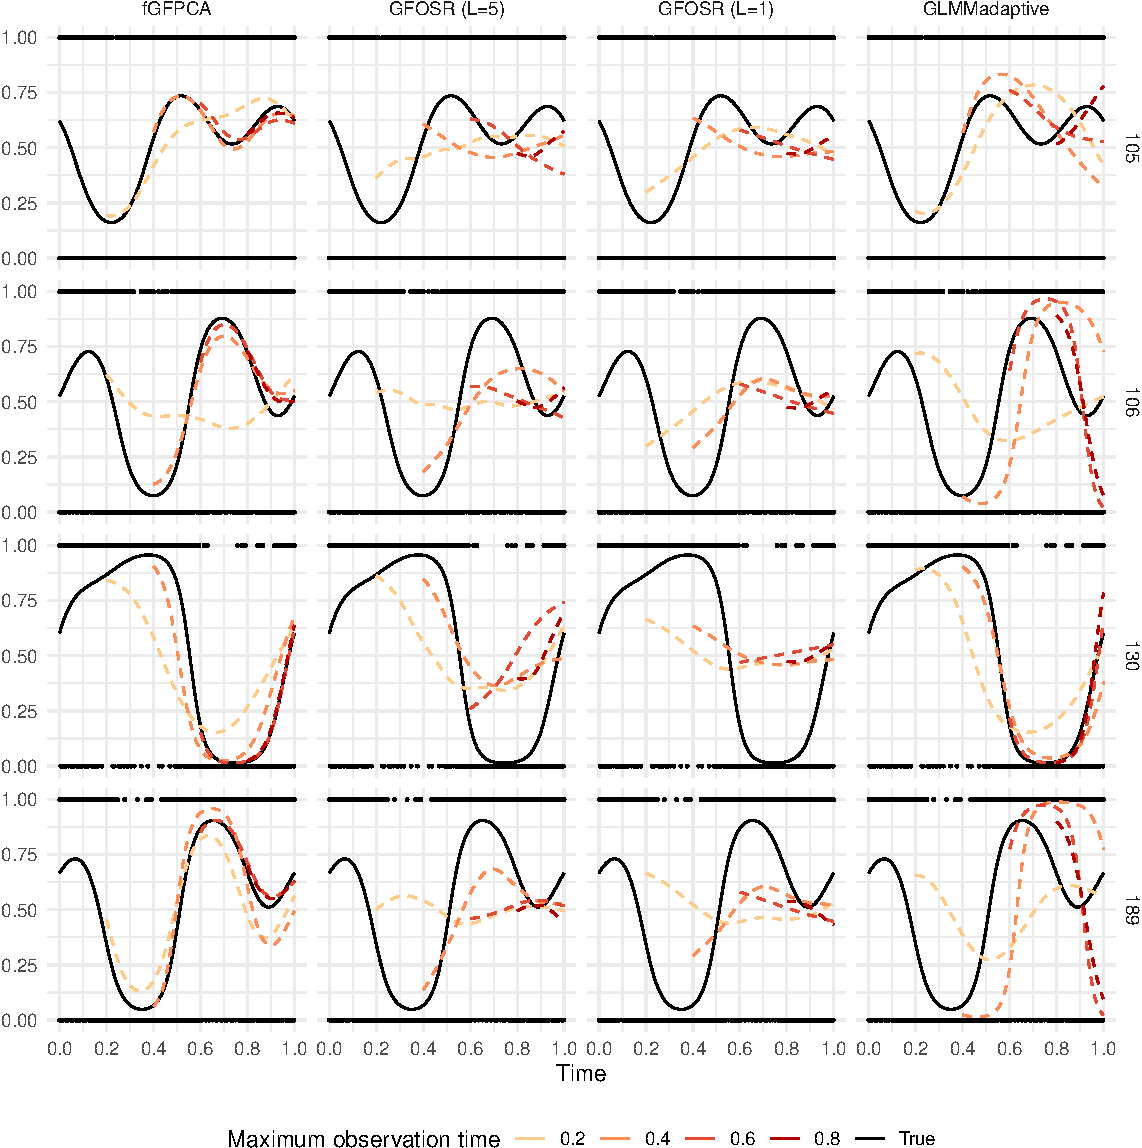
\includegraphics{manuscript_files/figure-latex/fig_small_sim-1.pdf}

\hypertarget{ise-and-auc-1}{%
\subsection{ISE and AUC}\label{ise-and-auc-1}}

\begin{Shaded}
\begin{Highlighting}[]
\DocumentationTok{\#\# ISE container }
\NormalTok{ise\_fgfpca2 }\OtherTok{\textless{}{-}}\NormalTok{ ise\_adglmm2 }\OtherTok{\textless{}{-}}\NormalTok{ ise\_gfosr\_l1\_2 }\OtherTok{\textless{}{-}}\NormalTok{ ise\_gfosr\_l5\_2 }\OtherTok{\textless{}{-}} 
  \FunctionTok{array}\NormalTok{(}\ConstantTok{NA}\NormalTok{, }\AttributeTok{dim =} \FunctionTok{c}\NormalTok{(}\FunctionTok{length}\NormalTok{(window)}\SpecialCharTok{{-}}\DecValTok{2}\NormalTok{, }\FunctionTok{length}\NormalTok{(window)}\SpecialCharTok{{-}}\DecValTok{2}\NormalTok{, M))}
\CommentTok{\# dims: prediction window, max obs time, simulation iter}
\end{Highlighting}
\end{Shaded}

\begin{Shaded}
\begin{Highlighting}[]
\ControlFlowTok{for}\NormalTok{(m }\ControlFlowTok{in} \DecValTok{1}\SpecialCharTok{:}\FunctionTok{length}\NormalTok{(pred\_subset\_fGFPCA))\{}
\NormalTok{  this\_df }\OtherTok{\textless{}{-}}\NormalTok{ pred\_subset\_fGFPCA[[m]]}
\NormalTok{  ise\_tb\_m }\OtherTok{\textless{}{-}}\NormalTok{ this\_df }\SpecialCharTok{\%\textgreater{}\%}
    \FunctionTok{mutate}\NormalTok{(}\AttributeTok{err1 =}\NormalTok{ (pred0}\FloatTok{.2}\SpecialCharTok{{-}}\NormalTok{eta\_i)}\SpecialCharTok{\^{}}\DecValTok{2}\NormalTok{,}
           \AttributeTok{err2 =}\NormalTok{ (pred0}\FloatTok{.4}\SpecialCharTok{{-}}\NormalTok{eta\_i)}\SpecialCharTok{\^{}}\DecValTok{2}\NormalTok{,}
           \AttributeTok{err3 =}\NormalTok{ (pred0}\FloatTok{.6}\SpecialCharTok{{-}}\NormalTok{eta\_i)}\SpecialCharTok{\^{}}\DecValTok{2}\NormalTok{,}
           \AttributeTok{err4 =}\NormalTok{ (pred0}\FloatTok{.8}\SpecialCharTok{{-}}\NormalTok{eta\_i)}\SpecialCharTok{\^{}}\DecValTok{2}\NormalTok{) }\SpecialCharTok{\%\textgreater{}\%}
    \FunctionTok{select}\NormalTok{(id, t, }\FunctionTok{starts\_with}\NormalTok{(}\StringTok{"err"}\NormalTok{)) }\SpecialCharTok{\%\textgreater{}\%} 
    \FunctionTok{mutate}\NormalTok{(}\AttributeTok{window =} \FunctionTok{cut}\NormalTok{(t, }\AttributeTok{breaks =}\NormalTok{ window, }\AttributeTok{include.lowest =}\NormalTok{ T)) }\SpecialCharTok{\%\textgreater{}\%} 
    \FunctionTok{group\_by}\NormalTok{(window, id) }\SpecialCharTok{\%\textgreater{}\%} 
    \FunctionTok{summarise\_at}\NormalTok{(}\FunctionTok{vars}\NormalTok{(err1, err2, err3, err4), sum) }\SpecialCharTok{\%\textgreater{}\%} 
    \FunctionTok{group\_by}\NormalTok{(window) }\SpecialCharTok{\%\textgreater{}\%} 
    \FunctionTok{summarize\_at}\NormalTok{(}\FunctionTok{vars}\NormalTok{(err1, err2, err3, err4), mean) }\SpecialCharTok{\%\textgreater{}\%}
    \FunctionTok{filter}\NormalTok{(window }\SpecialCharTok{!=} \StringTok{"[0,0.2]"}\NormalTok{) }\SpecialCharTok{\%\textgreater{}\%} 
    \FunctionTok{select}\NormalTok{(}\FunctionTok{starts\_with}\NormalTok{(}\StringTok{"err"}\NormalTok{)) }\SpecialCharTok{\%\textgreater{}\%} \FunctionTok{as.matrix}\NormalTok{()}
\NormalTok{  ise\_fgfpca2[,,m] }\OtherTok{\textless{}{-}}\NormalTok{ ise\_tb\_m}
\NormalTok{\}}

\NormalTok{mean\_ise\_fgfpca2 }\OtherTok{\textless{}{-}} \FunctionTok{apply}\NormalTok{(ise\_fgfpca2, }\FunctionTok{c}\NormalTok{(}\DecValTok{1}\NormalTok{, }\DecValTok{2}\NormalTok{), mean)}

\FunctionTok{colnames}\NormalTok{(mean\_ise\_fgfpca2) }\OtherTok{\textless{}{-}} \FunctionTok{c}\NormalTok{(}\StringTok{"0.2"}\NormalTok{, }\StringTok{"0.4"}\NormalTok{, }\StringTok{"0.6"}\NormalTok{, }\StringTok{"0.8"}\NormalTok{)}
\end{Highlighting}
\end{Shaded}

\begin{Shaded}
\begin{Highlighting}[]
\ControlFlowTok{for}\NormalTok{(m }\ControlFlowTok{in} \DecValTok{1}\SpecialCharTok{:}\FunctionTok{length}\NormalTok{(pred\_subset\_adglmm))\{}
\NormalTok{  this\_df }\OtherTok{\textless{}{-}}\NormalTok{ pred\_subset\_adglmm[[m]]}
\NormalTok{  ise\_tb\_m }\OtherTok{\textless{}{-}}\NormalTok{ this\_df }\SpecialCharTok{\%\textgreater{}\%}
    \FunctionTok{mutate}\NormalTok{(}\AttributeTok{err1 =}\NormalTok{ (pred0}\FloatTok{.2}\SpecialCharTok{{-}}\NormalTok{eta\_i)}\SpecialCharTok{\^{}}\DecValTok{2}\NormalTok{,}
           \AttributeTok{err2 =}\NormalTok{ (pred0}\FloatTok{.4}\SpecialCharTok{{-}}\NormalTok{eta\_i)}\SpecialCharTok{\^{}}\DecValTok{2}\NormalTok{,}
           \AttributeTok{err3 =}\NormalTok{ (pred0}\FloatTok{.6}\SpecialCharTok{{-}}\NormalTok{eta\_i)}\SpecialCharTok{\^{}}\DecValTok{2}\NormalTok{,}
           \AttributeTok{err4 =}\NormalTok{ (pred0}\FloatTok{.8}\SpecialCharTok{{-}}\NormalTok{eta\_i)}\SpecialCharTok{\^{}}\DecValTok{2}\NormalTok{) }\SpecialCharTok{\%\textgreater{}\%}
    \FunctionTok{select}\NormalTok{(id, t, }\FunctionTok{starts\_with}\NormalTok{(}\StringTok{"err"}\NormalTok{)) }\SpecialCharTok{\%\textgreater{}\%} 
    \FunctionTok{mutate}\NormalTok{(}\AttributeTok{window =} \FunctionTok{cut}\NormalTok{(t, }\AttributeTok{breaks =}\NormalTok{ window, }\AttributeTok{include.lowest =}\NormalTok{ T)) }\SpecialCharTok{\%\textgreater{}\%} 
    \FunctionTok{group\_by}\NormalTok{(window, id) }\SpecialCharTok{\%\textgreater{}\%} 
    \FunctionTok{summarise\_at}\NormalTok{(}\FunctionTok{vars}\NormalTok{(err1, err2, err3, err4), sum) }\SpecialCharTok{\%\textgreater{}\%} 
    \FunctionTok{group\_by}\NormalTok{(window) }\SpecialCharTok{\%\textgreater{}\%} 
    \FunctionTok{summarize\_at}\NormalTok{(}\FunctionTok{vars}\NormalTok{(err1, err2, err3, err4), mean) }\SpecialCharTok{\%\textgreater{}\%}
    \FunctionTok{filter}\NormalTok{(window }\SpecialCharTok{!=} \StringTok{"[0,0.2]"}\NormalTok{) }\SpecialCharTok{\%\textgreater{}\%} 
    \FunctionTok{select}\NormalTok{(}\FunctionTok{starts\_with}\NormalTok{(}\StringTok{"err"}\NormalTok{)) }\SpecialCharTok{\%\textgreater{}\%} \FunctionTok{as.matrix}\NormalTok{()}
\NormalTok{  ise\_adglmm2[,,m] }\OtherTok{\textless{}{-}}\NormalTok{ ise\_tb\_m}
\NormalTok{\}}

\NormalTok{mean\_ise\_adglmm2}\OtherTok{\textless{}{-}} \FunctionTok{apply}\NormalTok{(ise\_adglmm2, }\FunctionTok{c}\NormalTok{(}\DecValTok{1}\NormalTok{, }\DecValTok{2}\NormalTok{), mean, }\AttributeTok{na.rm =}\NormalTok{ T)}

\FunctionTok{colnames}\NormalTok{(mean\_ise\_adglmm2) }\OtherTok{\textless{}{-}} \FunctionTok{c}\NormalTok{(}\StringTok{"0.2"}\NormalTok{, }\StringTok{"0.4"}\NormalTok{, }\StringTok{"0.6"}\NormalTok{, }\StringTok{"0.8"}\NormalTok{)}
\end{Highlighting}
\end{Shaded}

\begin{Shaded}
\begin{Highlighting}[]
\ControlFlowTok{for}\NormalTok{(m }\ControlFlowTok{in} \DecValTok{1}\SpecialCharTok{:}\FunctionTok{length}\NormalTok{(pred\_subset\_gfosr\_l1))\{}
\NormalTok{  this\_df }\OtherTok{\textless{}{-}}\NormalTok{ pred\_subset\_gfosr\_l1[[m]]}
\NormalTok{  ise\_tb\_m }\OtherTok{\textless{}{-}}\NormalTok{ this\_df }\SpecialCharTok{\%\textgreater{}\%}
    \FunctionTok{mutate}\NormalTok{(}\AttributeTok{err1 =}\NormalTok{ (pred\_w1}\SpecialCharTok{{-}}\NormalTok{eta\_i)}\SpecialCharTok{\^{}}\DecValTok{2}\NormalTok{,}
           \AttributeTok{err2 =}\NormalTok{ (pred\_w2}\SpecialCharTok{{-}}\NormalTok{eta\_i)}\SpecialCharTok{\^{}}\DecValTok{2}\NormalTok{,}
           \AttributeTok{err3 =}\NormalTok{ (pred\_w3}\SpecialCharTok{{-}}\NormalTok{eta\_i)}\SpecialCharTok{\^{}}\DecValTok{2}\NormalTok{,}
           \AttributeTok{err4 =}\NormalTok{ (pred\_w4}\SpecialCharTok{{-}}\NormalTok{eta\_i)}\SpecialCharTok{\^{}}\DecValTok{2}\NormalTok{) }\SpecialCharTok{\%\textgreater{}\%}
    \FunctionTok{select}\NormalTok{(id, t, }\FunctionTok{starts\_with}\NormalTok{(}\StringTok{"err"}\NormalTok{), window) }\SpecialCharTok{\%\textgreater{}\%} 
    \FunctionTok{group\_by}\NormalTok{(window, id) }\SpecialCharTok{\%\textgreater{}\%} 
    \FunctionTok{summarise\_at}\NormalTok{(}\FunctionTok{vars}\NormalTok{(err1, err2, err3, err4), sum) }\SpecialCharTok{\%\textgreater{}\%} 
    \FunctionTok{group\_by}\NormalTok{(window) }\SpecialCharTok{\%\textgreater{}\%} 
    \FunctionTok{summarize\_at}\NormalTok{(}\FunctionTok{vars}\NormalTok{(err1, err2, err3, err4), mean) }\SpecialCharTok{\%\textgreater{}\%}
    \FunctionTok{filter}\NormalTok{(window }\SpecialCharTok{!=} \DecValTok{1}\NormalTok{) }\SpecialCharTok{\%\textgreater{}\%} 
    \FunctionTok{select}\NormalTok{(}\FunctionTok{starts\_with}\NormalTok{(}\StringTok{"err"}\NormalTok{)) }\SpecialCharTok{\%\textgreater{}\%} \FunctionTok{as.matrix}\NormalTok{()}
\NormalTok{  ise\_gfosr\_l1\_2[,,m] }\OtherTok{\textless{}{-}}\NormalTok{ ise\_tb\_m}
\NormalTok{\}}

\NormalTok{mean\_ise\_gfosr\_l1\_2}\OtherTok{\textless{}{-}} \FunctionTok{apply}\NormalTok{(ise\_gfosr\_l1\_2, }\FunctionTok{c}\NormalTok{(}\DecValTok{1}\NormalTok{, }\DecValTok{2}\NormalTok{), mean, }\AttributeTok{na.rm =}\NormalTok{ T)}

\FunctionTok{colnames}\NormalTok{(mean\_ise\_gfosr\_l1\_2) }\OtherTok{\textless{}{-}} \FunctionTok{c}\NormalTok{(}\StringTok{"0.2"}\NormalTok{, }\StringTok{"0.4"}\NormalTok{, }\StringTok{"0.6"}\NormalTok{, }\StringTok{"0.8"}\NormalTok{)}
\end{Highlighting}
\end{Shaded}

\begin{Shaded}
\begin{Highlighting}[]
\ControlFlowTok{for}\NormalTok{(m }\ControlFlowTok{in} \DecValTok{1}\SpecialCharTok{:}\FunctionTok{length}\NormalTok{(pred\_subset\_gfosr\_l5))\{}
\NormalTok{  this\_df }\OtherTok{\textless{}{-}}\NormalTok{ pred\_subset\_gfosr\_l5[[m]]}
\NormalTok{  ise\_tb\_m }\OtherTok{\textless{}{-}}\NormalTok{ this\_df }\SpecialCharTok{\%\textgreater{}\%}
    \FunctionTok{mutate}\NormalTok{(}\AttributeTok{err1 =}\NormalTok{ (pred\_w1}\SpecialCharTok{{-}}\NormalTok{eta\_i)}\SpecialCharTok{\^{}}\DecValTok{2}\NormalTok{,}
           \AttributeTok{err2 =}\NormalTok{ (pred\_w2}\SpecialCharTok{{-}}\NormalTok{eta\_i)}\SpecialCharTok{\^{}}\DecValTok{2}\NormalTok{,}
           \AttributeTok{err3 =}\NormalTok{ (pred\_w3}\SpecialCharTok{{-}}\NormalTok{eta\_i)}\SpecialCharTok{\^{}}\DecValTok{2}\NormalTok{,}
           \AttributeTok{err4 =}\NormalTok{ (pred\_w4}\SpecialCharTok{{-}}\NormalTok{eta\_i)}\SpecialCharTok{\^{}}\DecValTok{2}\NormalTok{) }\SpecialCharTok{\%\textgreater{}\%}
    \FunctionTok{select}\NormalTok{(id, t, }\FunctionTok{starts\_with}\NormalTok{(}\StringTok{"err"}\NormalTok{), window) }\SpecialCharTok{\%\textgreater{}\%} 
    \FunctionTok{group\_by}\NormalTok{(window, id) }\SpecialCharTok{\%\textgreater{}\%} 
    \FunctionTok{summarise\_at}\NormalTok{(}\FunctionTok{vars}\NormalTok{(err1, err2, err3, err4), sum) }\SpecialCharTok{\%\textgreater{}\%} 
    \FunctionTok{group\_by}\NormalTok{(window) }\SpecialCharTok{\%\textgreater{}\%} 
    \FunctionTok{summarize\_at}\NormalTok{(}\FunctionTok{vars}\NormalTok{(err1, err2, err3, err4), mean) }\SpecialCharTok{\%\textgreater{}\%}
    \FunctionTok{filter}\NormalTok{(window }\SpecialCharTok{!=} \DecValTok{1}\NormalTok{) }\SpecialCharTok{\%\textgreater{}\%} 
    \FunctionTok{select}\NormalTok{(}\FunctionTok{starts\_with}\NormalTok{(}\StringTok{"err"}\NormalTok{)) }\SpecialCharTok{\%\textgreater{}\%} \FunctionTok{as.matrix}\NormalTok{()}
\NormalTok{  ise\_gfosr\_l5\_2[,,m] }\OtherTok{\textless{}{-}}\NormalTok{ ise\_tb\_m}
\NormalTok{\}}

\NormalTok{mean\_ise\_gfosr\_l5\_2 }\OtherTok{\textless{}{-}} \FunctionTok{apply}\NormalTok{(ise\_gfosr\_l5\_2, }\FunctionTok{c}\NormalTok{(}\DecValTok{1}\NormalTok{, }\DecValTok{2}\NormalTok{), mean, }\AttributeTok{na.rm =}\NormalTok{ T)}

\FunctionTok{colnames}\NormalTok{(mean\_ise\_gfosr\_l5\_2) }\OtherTok{\textless{}{-}} \FunctionTok{c}\NormalTok{(}\StringTok{"0.2"}\NormalTok{, }\StringTok{"0.4"}\NormalTok{, }\StringTok{"0.6"}\NormalTok{, }\StringTok{"0.8"}\NormalTok{)}
\end{Highlighting}
\end{Shaded}

\begin{Shaded}
\begin{Highlighting}[]
\DocumentationTok{\#\# auc container }
\NormalTok{auc\_fgfpca2 }\OtherTok{\textless{}{-}}\NormalTok{ auc\_adglmm2 }\OtherTok{\textless{}{-}}\NormalTok{ auc\_gfosr\_l1\_2 }\OtherTok{\textless{}{-}}\NormalTok{ auc\_gfosr\_l5\_2 }\OtherTok{\textless{}{-}} 
  \FunctionTok{array}\NormalTok{(}\ConstantTok{NA}\NormalTok{, }\AttributeTok{dim =} \FunctionTok{c}\NormalTok{(}\FunctionTok{length}\NormalTok{(window)}\SpecialCharTok{{-}}\DecValTok{2}\NormalTok{, }\FunctionTok{length}\NormalTok{(window)}\SpecialCharTok{{-}}\DecValTok{2}\NormalTok{, M))}
\end{Highlighting}
\end{Shaded}

\begin{Shaded}
\begin{Highlighting}[]
\ControlFlowTok{for}\NormalTok{(m }\ControlFlowTok{in} \DecValTok{1}\SpecialCharTok{:}\FunctionTok{length}\NormalTok{(pred\_subset\_fGFPCA))\{}
\NormalTok{  this\_df }\OtherTok{\textless{}{-}}\NormalTok{ pred\_subset\_fGFPCA[[m]]}
\NormalTok{  auc\_tb\_m }\OtherTok{\textless{}{-}}\NormalTok{ this\_df }\SpecialCharTok{\%\textgreater{}\%}
  \FunctionTok{mutate}\NormalTok{(}\AttributeTok{window =} \FunctionTok{cut}\NormalTok{(t, }\AttributeTok{breaks =}\NormalTok{ window, }\AttributeTok{include.lowest =}\NormalTok{ T)) }\SpecialCharTok{\%\textgreater{}\%} 
  \FunctionTok{select}\NormalTok{(Y, }\FunctionTok{starts\_with}\NormalTok{(}\StringTok{"pred"}\NormalTok{), window) }\SpecialCharTok{\%\textgreater{}\%}
  \FunctionTok{group\_by}\NormalTok{(window) }\SpecialCharTok{\%\textgreater{}\%}
  \FunctionTok{summarise}\NormalTok{(}\AttributeTok{auc1 =} \FunctionTok{get\_auc}\NormalTok{(Y, pred0}\FloatTok{.2}\NormalTok{),}
            \AttributeTok{auc2 =} \FunctionTok{get\_auc}\NormalTok{(Y, pred0}\FloatTok{.4}\NormalTok{),}
            \AttributeTok{auc3 =} \FunctionTok{get\_auc}\NormalTok{(Y, pred0}\FloatTok{.6}\NormalTok{),}
            \AttributeTok{auc4 =} \FunctionTok{get\_auc}\NormalTok{(Y, pred0}\FloatTok{.8}\NormalTok{)) }\SpecialCharTok{\%\textgreater{}\%}
  \FunctionTok{filter}\NormalTok{(window }\SpecialCharTok{!=} \StringTok{"[0,0.2]"}\NormalTok{) }\SpecialCharTok{\%\textgreater{}\%} 
  \FunctionTok{select}\NormalTok{(}\FunctionTok{starts\_with}\NormalTok{(}\StringTok{"auc"}\NormalTok{)) }\SpecialCharTok{\%\textgreater{}\%} \FunctionTok{as.matrix}\NormalTok{()}
  
\NormalTok{  auc\_fgfpca2[, , m] }\OtherTok{\textless{}{-}}\NormalTok{ auc\_tb\_m}
  
\NormalTok{\}}

\NormalTok{mean\_auc\_fgfpca2 }\OtherTok{\textless{}{-}} \FunctionTok{apply}\NormalTok{(auc\_fgfpca2, }\FunctionTok{c}\NormalTok{(}\DecValTok{1}\NormalTok{,}\DecValTok{2}\NormalTok{), mean)}
\FunctionTok{colnames}\NormalTok{(mean\_auc\_fgfpca2) }\OtherTok{\textless{}{-}} \FunctionTok{c}\NormalTok{(}\StringTok{"0.2"}\NormalTok{, }\StringTok{"0.4"}\NormalTok{, }\StringTok{"0.6"}\NormalTok{, }\StringTok{"0.8"}\NormalTok{)}
\end{Highlighting}
\end{Shaded}

\begin{Shaded}
\begin{Highlighting}[]
\ControlFlowTok{for}\NormalTok{(m }\ControlFlowTok{in} \DecValTok{1}\SpecialCharTok{:}\FunctionTok{length}\NormalTok{(pred\_subset\_adglmm))\{}
\NormalTok{  this\_df }\OtherTok{\textless{}{-}}\NormalTok{ pred\_subset\_adglmm[[m]]}
\NormalTok{  auc\_tb\_m }\OtherTok{\textless{}{-}}\NormalTok{ this\_df }\SpecialCharTok{\%\textgreater{}\%}
  \FunctionTok{mutate}\NormalTok{(}\AttributeTok{window =} \FunctionTok{cut}\NormalTok{(t, }\AttributeTok{breaks =}\NormalTok{ window, }\AttributeTok{include.lowest =}\NormalTok{ T)) }\SpecialCharTok{\%\textgreater{}\%} 
  \FunctionTok{select}\NormalTok{(Y, }\FunctionTok{starts\_with}\NormalTok{(}\StringTok{"pred"}\NormalTok{), window) }\SpecialCharTok{\%\textgreater{}\%}
  \FunctionTok{group\_by}\NormalTok{(window) }\SpecialCharTok{\%\textgreater{}\%}
  \FunctionTok{summarise}\NormalTok{(}\AttributeTok{auc1 =} \FunctionTok{get\_auc}\NormalTok{(Y, pred0}\FloatTok{.2}\NormalTok{),}
            \AttributeTok{auc2 =} \FunctionTok{get\_auc}\NormalTok{(Y, pred0}\FloatTok{.4}\NormalTok{),}
            \AttributeTok{auc3 =} \FunctionTok{get\_auc}\NormalTok{(Y, pred0}\FloatTok{.6}\NormalTok{),}
            \AttributeTok{auc4 =} \FunctionTok{get\_auc}\NormalTok{(Y, pred0}\FloatTok{.8}\NormalTok{)) }\SpecialCharTok{\%\textgreater{}\%}
  \FunctionTok{filter}\NormalTok{(window }\SpecialCharTok{!=} \StringTok{"[0,0.2]"}\NormalTok{) }\SpecialCharTok{\%\textgreater{}\%} 
  \FunctionTok{select}\NormalTok{(}\FunctionTok{starts\_with}\NormalTok{(}\StringTok{"auc"}\NormalTok{)) }\SpecialCharTok{\%\textgreater{}\%} \FunctionTok{as.matrix}\NormalTok{()}
  
\NormalTok{  auc\_adglmm2[, , m] }\OtherTok{\textless{}{-}}\NormalTok{ auc\_tb\_m}
  
\NormalTok{\}}

\NormalTok{mean\_auc\_adglmm2 }\OtherTok{\textless{}{-}} \FunctionTok{apply}\NormalTok{(auc\_adglmm2, }\FunctionTok{c}\NormalTok{(}\DecValTok{1}\NormalTok{,}\DecValTok{2}\NormalTok{), mean, }\AttributeTok{na.rm =}\NormalTok{ T)}
\FunctionTok{colnames}\NormalTok{(mean\_auc\_adglmm2) }\OtherTok{\textless{}{-}} \FunctionTok{c}\NormalTok{(}\StringTok{"0.2"}\NormalTok{, }\StringTok{"0.4"}\NormalTok{, }\StringTok{"0.6"}\NormalTok{, }\StringTok{"0.8"}\NormalTok{)}
\end{Highlighting}
\end{Shaded}

\begin{Shaded}
\begin{Highlighting}[]
\ControlFlowTok{for}\NormalTok{(m }\ControlFlowTok{in} \DecValTok{1}\SpecialCharTok{:}\FunctionTok{length}\NormalTok{(pred\_subset\_gfosr\_l1))\{}
\NormalTok{  this\_df }\OtherTok{\textless{}{-}}\NormalTok{ pred\_subset\_gfosr\_l1[[m]]}
\NormalTok{  auc\_tb\_m }\OtherTok{\textless{}{-}}\NormalTok{ this\_df }\SpecialCharTok{\%\textgreater{}\%}
  \FunctionTok{select}\NormalTok{(Y, }\FunctionTok{starts\_with}\NormalTok{(}\StringTok{"pred"}\NormalTok{), window) }\SpecialCharTok{\%\textgreater{}\%}
  \FunctionTok{group\_by}\NormalTok{(window) }\SpecialCharTok{\%\textgreater{}\%}
  \FunctionTok{summarise}\NormalTok{(}\AttributeTok{auc1 =} \FunctionTok{get\_auc}\NormalTok{(Y, pred\_w1),}
            \AttributeTok{auc2 =} \FunctionTok{get\_auc}\NormalTok{(Y, pred\_w2),}
            \AttributeTok{auc3 =} \FunctionTok{get\_auc}\NormalTok{(Y, pred\_w3),}
            \AttributeTok{auc4 =} \FunctionTok{get\_auc}\NormalTok{(Y, pred\_w4)) }\SpecialCharTok{\%\textgreater{}\%}
  \FunctionTok{filter}\NormalTok{(window }\SpecialCharTok{!=} \DecValTok{1}\NormalTok{) }\SpecialCharTok{\%\textgreater{}\%} 
  \FunctionTok{select}\NormalTok{(}\FunctionTok{starts\_with}\NormalTok{(}\StringTok{"auc"}\NormalTok{)) }\SpecialCharTok{\%\textgreater{}\%} \FunctionTok{as.matrix}\NormalTok{()}
  
\NormalTok{  auc\_gfosr\_l1\_2[, , m] }\OtherTok{\textless{}{-}}\NormalTok{ auc\_tb\_m}
  
\NormalTok{\}}

\NormalTok{mean\_auc\_gfosr\_l1\_2 }\OtherTok{\textless{}{-}} \FunctionTok{apply}\NormalTok{(auc\_gfosr\_l1\_2, }\FunctionTok{c}\NormalTok{(}\DecValTok{1}\NormalTok{,}\DecValTok{2}\NormalTok{), mean)}
\FunctionTok{colnames}\NormalTok{(mean\_auc\_gfosr\_l1\_2) }\OtherTok{\textless{}{-}} \FunctionTok{c}\NormalTok{(}\StringTok{"0.2"}\NormalTok{, }\StringTok{"0.4"}\NormalTok{, }\StringTok{"0.6"}\NormalTok{, }\StringTok{"0.8"}\NormalTok{)}
\end{Highlighting}
\end{Shaded}

\begin{Shaded}
\begin{Highlighting}[]
\ControlFlowTok{for}\NormalTok{(m }\ControlFlowTok{in} \DecValTok{1}\SpecialCharTok{:}\FunctionTok{length}\NormalTok{(pred\_subset\_gfosr\_l5))\{}
\NormalTok{  this\_df }\OtherTok{\textless{}{-}}\NormalTok{ pred\_subset\_gfosr\_l5[[m]]}
\NormalTok{  auc\_tb\_m }\OtherTok{\textless{}{-}}\NormalTok{ this\_df }\SpecialCharTok{\%\textgreater{}\%}
  \FunctionTok{select}\NormalTok{(Y, }\FunctionTok{starts\_with}\NormalTok{(}\StringTok{"pred"}\NormalTok{), window) }\SpecialCharTok{\%\textgreater{}\%}
  \FunctionTok{group\_by}\NormalTok{(window) }\SpecialCharTok{\%\textgreater{}\%}
  \FunctionTok{summarise}\NormalTok{(}\AttributeTok{auc1 =} \FunctionTok{get\_auc}\NormalTok{(Y, pred\_w1),}
            \AttributeTok{auc2 =} \FunctionTok{get\_auc}\NormalTok{(Y, pred\_w2),}
            \AttributeTok{auc3 =} \FunctionTok{get\_auc}\NormalTok{(Y, pred\_w3),}
            \AttributeTok{auc4 =} \FunctionTok{get\_auc}\NormalTok{(Y, pred\_w4)) }\SpecialCharTok{\%\textgreater{}\%}
  \FunctionTok{filter}\NormalTok{(window }\SpecialCharTok{!=} \DecValTok{1}\NormalTok{) }\SpecialCharTok{\%\textgreater{}\%} 
  \FunctionTok{select}\NormalTok{(}\FunctionTok{starts\_with}\NormalTok{(}\StringTok{"auc"}\NormalTok{)) }\SpecialCharTok{\%\textgreater{}\%} \FunctionTok{as.matrix}\NormalTok{()}
  
\NormalTok{  auc\_gfosr\_l5\_2[, , m] }\OtherTok{\textless{}{-}}\NormalTok{ auc\_tb\_m}
  
\NormalTok{\}}

\NormalTok{mean\_auc\_gfosr\_l5\_2 }\OtherTok{\textless{}{-}} \FunctionTok{apply}\NormalTok{(auc\_gfosr\_l5\_2, }\FunctionTok{c}\NormalTok{(}\DecValTok{1}\NormalTok{,}\DecValTok{2}\NormalTok{), mean)}
\FunctionTok{colnames}\NormalTok{(mean\_auc\_gfosr\_l5\_2) }\OtherTok{\textless{}{-}} \FunctionTok{c}\NormalTok{(}\StringTok{"0.2"}\NormalTok{, }\StringTok{"0.4"}\NormalTok{, }\StringTok{"0.6"}\NormalTok{, }\StringTok{"0.8"}\NormalTok{)}
\end{Highlighting}
\end{Shaded}

\begin{Shaded}
\begin{Highlighting}[]
\NormalTok{fgfpca2 }\OtherTok{\textless{}{-}} \FunctionTok{rbind}\NormalTok{(mean\_ise\_fgfpca2 ,mean\_auc\_fgfpca2) }\SpecialCharTok{\%\textgreater{}\%} \FunctionTok{as\_tibble}\NormalTok{() }\SpecialCharTok{\%\textgreater{}\%}
  \FunctionTok{mutate}\NormalTok{(}\AttributeTok{Window =} \FunctionTok{rep}\NormalTok{(}\FunctionTok{c}\NormalTok{(}\StringTok{"(0.2, 0.4]"}\NormalTok{, }\StringTok{"(0.4, 0.6]"}\NormalTok{, }\StringTok{"(0.6, 0.8]"}\NormalTok{, }\StringTok{"(0.8, 1.0]"}\NormalTok{), }\DecValTok{2}\NormalTok{), }\AttributeTok{.before=}\DecValTok{1}\NormalTok{)}
\NormalTok{gfosr\_l5\_2 }\OtherTok{\textless{}{-}} \FunctionTok{rbind}\NormalTok{(mean\_ise\_gfosr\_l5\_2 ,mean\_auc\_gfosr\_l5\_2) }\SpecialCharTok{\%\textgreater{}\%} \FunctionTok{as\_tibble}\NormalTok{()}
\NormalTok{gfosr\_l1\_2 }\OtherTok{\textless{}{-}} \FunctionTok{rbind}\NormalTok{(mean\_ise\_gfosr\_l1\_2 ,mean\_auc\_gfosr\_l1\_2) }\SpecialCharTok{\%\textgreater{}\%} \FunctionTok{as\_tibble}\NormalTok{()}
\NormalTok{adglmm2 }\OtherTok{\textless{}{-}} \FunctionTok{rbind}\NormalTok{(mean\_ise\_adglmm2 ,mean\_auc\_adglmm2) }\SpecialCharTok{\%\textgreater{}\%} \FunctionTok{as\_tibble}\NormalTok{() }

\FunctionTok{bind\_cols}\NormalTok{(fgfpca2, gfosr\_l5\_2, gfosr\_l1\_2, adglmm2, }\AttributeTok{.name\_repair =} \StringTok{"minimal"}\NormalTok{) }\SpecialCharTok{\%\textgreater{}\%}
  \FunctionTok{kable}\NormalTok{(}\AttributeTok{digits =} \DecValTok{3}\NormalTok{, }\AttributeTok{booktabs=}\NormalTok{T,}
        \AttributeTok{table.attr=}\StringTok{"style=}\SpecialCharTok{\textbackslash{}"}\StringTok{color:black;}\SpecialCharTok{\textbackslash{}"}\StringTok{"}\NormalTok{) }\SpecialCharTok{\%\textgreater{}\%}
  \FunctionTok{kable\_styling}\NormalTok{(}\AttributeTok{full\_width =}\NormalTok{ F) }\SpecialCharTok{\%\textgreater{}\%} 
  \FunctionTok{add\_header\_above}\NormalTok{(}\FunctionTok{c}\NormalTok{(}\StringTok{" "} \OtherTok{=} \DecValTok{1}\NormalTok{, }\StringTok{"fGFPCA"} \OtherTok{=} \DecValTok{4}\NormalTok{, }\StringTok{"GFOSR (L=5)"} \OtherTok{=} \DecValTok{4}\NormalTok{, }
                     \StringTok{"GFOSR (L=1)"} \OtherTok{=} \DecValTok{4}\NormalTok{, }\StringTok{"GLMMadaptive"} \OtherTok{=} \DecValTok{4}\NormalTok{)) }\SpecialCharTok{\%\textgreater{}\%}
  \FunctionTok{add\_header\_above}\NormalTok{(}\FunctionTok{c}\NormalTok{(}\StringTok{" "} \OtherTok{=} \DecValTok{1}\NormalTok{, }\StringTok{"Maximum observation time"} \OtherTok{=} \DecValTok{16}\NormalTok{)) }\SpecialCharTok{\%\textgreater{}\%}
  \FunctionTok{group\_rows}\NormalTok{(}\AttributeTok{index =} \FunctionTok{c}\NormalTok{(}\StringTok{"ISE"}\OtherTok{=} \DecValTok{4}\NormalTok{, }\StringTok{"AUC"} \OtherTok{=} \DecValTok{4}\NormalTok{)) }\SpecialCharTok{\%\textgreater{}\%}
  \FunctionTok{landscape}\NormalTok{()}
\end{Highlighting}
\end{Shaded}

\begin{landscape}\begin{table}
\centering
\begin{tabular}{lrrrrrrrrrrrrrrrr}
\toprule
\multicolumn{1}{c}{ } & \multicolumn{16}{c}{Maximum observation time} \\
\cmidrule(l{3pt}r{3pt}){2-17}
\multicolumn{1}{c}{ } & \multicolumn{4}{c}{fGFPCA} & \multicolumn{4}{c}{GFOSR (L=5)} & \multicolumn{4}{c}{GFOSR (L=1)} & \multicolumn{4}{c}{GLMMadaptive} \\
\cmidrule(l{3pt}r{3pt}){2-5} \cmidrule(l{3pt}r{3pt}){6-9} \cmidrule(l{3pt}r{3pt}){10-13} \cmidrule(l{3pt}r{3pt}){14-17}
Window & 0.2 & 0.4 & 0.6 & 0.8 & 0.2 & 0.4 & 0.6 & 0.8 & 0.2 & 0.4 & 0.6 & 0.8 & 0.2 & 0.4 & 0.6 & 0.8\\
\midrule
\addlinespace[0.3em]
\multicolumn{17}{l}{\textbf{ISE}}\\
\hspace{1em}(0.2, 0.4] & 150.641 &  &  &  & 286.853 &  &  &  & 367.282 &  &  &  & 374.836 &  &  & \\
\hspace{1em}(0.4, 0.6] & 188.065 & 77.380 &  &  & 286.628 & 227.225 &  &  & 290.781 & 265.809 &  &  & 268.390 & 463.337 &  & \\
\hspace{1em}(0.6, 0.8] & 224.001 & 51.533 & 16.879 &  & 328.612 & 374.572 & 326.522 &  & 386.705 & 408.427 & 388.427 &  & 319.731 & 287.001 & 233.510 & \\
\hspace{1em}(0.8, 1.0] & 112.163 & 81.368 & 19.592 & 13.399 & 301.165 & 324.817 & 353.888 & 335.139 & 331.488 & 342.935 & 354.800 & 347.627 & 228.335 & 469.769 & 331.509 & 131.993\\
\addlinespace[0.3em]
\multicolumn{17}{l}{\textbf{AUC}}\\
\hspace{1em}(0.2, 0.4] & 0.746 &  &  &  & 0.679 &  &  &  & 0.620 &  &  &  & 0.672 &  &  & \\
\hspace{1em}(0.4, 0.6] & 0.662 & 0.734 &  &  & 0.549 & 0.627 &  &  & 0.536 & 0.590 &  &  & 0.622 & 0.671 &  & \\
\hspace{1em}(0.6, 0.8] & 0.710 & 0.787 & 0.801 &  & 0.656 & 0.617 & 0.668 &  & 0.598 & 0.574 & 0.613 &  & 0.689 & 0.698 & 0.731 & \\
\hspace{1em}(0.8, 1.0] & 0.740 & 0.754 & 0.781 & 0.784 & 0.611 & 0.588 & 0.551 & 0.578 & 0.580 & 0.556 & 0.536 & 0.551 & 0.681 & 0.629 & 0.679 & 0.743\\
\bottomrule
\end{tabular}
\end{table}
\end{landscape}

Among 500 hundred iterations, 6 did not converge for the GLMMadaptive
model. No numeric issue for fGFPCA.

\hypertarget{time}{%
\section{Time}\label{time}}

\begin{Shaded}
\begin{Highlighting}[]
\FunctionTok{data.frame}\NormalTok{(}
  \StringTok{"Method"} \OtherTok{=} \FunctionTok{c}\NormalTok{(}\StringTok{"fGFPCA"}\NormalTok{, }\StringTok{"GLMMadaptive"}\NormalTok{, }\StringTok{"GFOSR (L=1)"}\NormalTok{, }\StringTok{"GFOSR (L=5)"}\NormalTok{),}
  \StringTok{"Time"} \OtherTok{=} \FunctionTok{c}\NormalTok{(}\FunctionTok{mean}\NormalTok{(fit\_time\_subset\_fGFPCA}\SpecialCharTok{/}\DecValTok{60}\SpecialCharTok{+}\NormalTok{pred\_time\_subset\_fGFPCA),}
             \FunctionTok{mean}\NormalTok{(fit\_time\_subset\_adglmm}\SpecialCharTok{+}\NormalTok{pred\_time\_subset\_adglmm}\SpecialCharTok{/}\DecValTok{60}\NormalTok{),}
             \FunctionTok{mean}\NormalTok{(t\_subset\_gfosr\_l1}\SpecialCharTok{/}\DecValTok{60}\NormalTok{), }
             \FunctionTok{mean}\NormalTok{(t\_subset\_gfosr\_l5}\SpecialCharTok{/}\DecValTok{60}\NormalTok{))) }\SpecialCharTok{\%\textgreater{}\%}
  \FunctionTok{kable}\NormalTok{(}\AttributeTok{digits =} \DecValTok{3}\NormalTok{, }\AttributeTok{booktabs =}\NormalTok{ T, }\AttributeTok{table.attr =} \StringTok{"style = }\SpecialCharTok{\textbackslash{}"}\StringTok{color:black;}\SpecialCharTok{\textbackslash{}"}\StringTok{"}\NormalTok{) }\SpecialCharTok{\%\textgreater{}\%}
  \FunctionTok{kable\_styling}\NormalTok{(}\AttributeTok{full\_width =}\NormalTok{ F) }
\end{Highlighting}
\end{Shaded}

\begin{table}
\centering
\begin{tabular}{lr}
\toprule
Method & Time\\
\midrule
fGFPCA & 1.629\\
GLMMadaptive & 5.479\\
GFOSR (L=1) & 0.010\\
GFOSR (L=5) & 0.054\\
\bottomrule
\end{tabular}
\end{table}

\hypertarget{nhanes-data-application}{%
\section{NHANES data application}\label{nhanes-data-application}}

We take 60\% subjects (N = 5257) for training, 40\% (n = 3506) for
out-of-sample prediction. When using the full sample The debiase step
(mgcv::bam) in fGFPCA took a really a long time, and GLMM adaptive only
works for intercept-only model. In the debias step, re-evaluated
eigenvalues also lost their decreasing nature.

\begin{Shaded}
\begin{Highlighting}[]
\CommentTok{\# df\_nhanes \textless{}{-} read\_rds(here("Data/nhanes\_bi.rds"))}
\FunctionTok{load}\NormalTok{(}\FunctionTok{here}\NormalTok{(}\StringTok{"Data/ApplOutput\_fGFPCA.RData"}\NormalTok{))}
\FunctionTok{load}\NormalTok{(}\FunctionTok{here}\NormalTok{(}\StringTok{"Data/ApplOutput\_GLMMadaptive.RData"}\NormalTok{))}

\FunctionTok{load}\NormalTok{(}\FunctionTok{here}\NormalTok{(}\StringTok{"Data/Appl\_GFOSR\_L5.RData"}\NormalTok{))}
\FunctionTok{load}\NormalTok{(}\FunctionTok{here}\NormalTok{(}\StringTok{"Data/Appl\_GFOSR\_L1.RData"}\NormalTok{))}

\NormalTok{pred\_appl\_gfosr\_l1 }\OtherTok{\textless{}{-}}\NormalTok{ pred\_appl\_gfosr\_l1 }\SpecialCharTok{\%\textgreater{}\%}
  \FunctionTok{rename}\NormalTok{(}\AttributeTok{pred360=}\NormalTok{pred\_w1, }\AttributeTok{pred720=}\NormalTok{pred\_w2, }\AttributeTok{pred1080=}\NormalTok{pred\_w3)}
\NormalTok{pred\_appl\_gfosr\_l5 }\OtherTok{\textless{}{-}}\NormalTok{ pred\_appl\_gfosr\_l5 }\SpecialCharTok{\%\textgreater{}\%}
  \FunctionTok{rename}\NormalTok{(}\AttributeTok{pred360=}\NormalTok{pred\_w1, }\AttributeTok{pred720=}\NormalTok{pred\_w2, }\AttributeTok{pred1080=}\NormalTok{pred\_w3)}
\end{Highlighting}
\end{Shaded}

\begin{Shaded}
\begin{Highlighting}[]
\NormalTok{df\_nhanes }\SpecialCharTok{\%\textgreater{}\%} \FunctionTok{select}\NormalTok{(SEQN, Z, sind) }\SpecialCharTok{\%\textgreater{}\%} 
  \FunctionTok{filter}\NormalTok{(SEQN }\SpecialCharTok{\%in\%} \FunctionTok{unique}\NormalTok{(nhanes\_pred\_adglmm}\SpecialCharTok{$}\NormalTok{id) }\SpecialCharTok{|}\NormalTok{ SEQN }\SpecialCharTok{\%in\%} \FunctionTok{unique}\NormalTok{(nhanes\_pred\_fgfpca}\SpecialCharTok{$}\NormalTok{id)) }\SpecialCharTok{\%\textgreater{}\%}
  \FunctionTok{mutate}\NormalTok{(}\AttributeTok{Z =} \FunctionTok{factor}\NormalTok{(Z, }\AttributeTok{levels =} \DecValTok{0}\SpecialCharTok{:}\DecValTok{1}\NormalTok{, }\AttributeTok{labels =} \FunctionTok{c}\NormalTok{(}\StringTok{"Inactive"}\NormalTok{, }\StringTok{"Active"}\NormalTok{))) }\SpecialCharTok{\%\textgreater{}\%}
  \FunctionTok{mutate}\NormalTok{(}\AttributeTok{SEQN =} \FunctionTok{factor}\NormalTok{(SEQN)) }\SpecialCharTok{\%\textgreater{}\%}
  \FunctionTok{ggplot}\NormalTok{()}\SpecialCharTok{+}
  \FunctionTok{geom\_tile}\NormalTok{(}\FunctionTok{aes}\NormalTok{(}\AttributeTok{x=}\NormalTok{sind, }\AttributeTok{y =}\NormalTok{ SEQN, }\AttributeTok{fill =}\NormalTok{ Z))}\SpecialCharTok{+}
  \FunctionTok{labs}\NormalTok{(}\AttributeTok{x=}\StringTok{"Time"}\NormalTok{, }\AttributeTok{y=}\StringTok{"Subject"}\NormalTok{, }\AttributeTok{title =} \StringTok{"Overview of NHANES binary activity indicator"}\NormalTok{)}\SpecialCharTok{+}
  \FunctionTok{theme}\NormalTok{(}\AttributeTok{axis.text.y =} \FunctionTok{element\_blank}\NormalTok{())}\SpecialCharTok{+}
  \FunctionTok{scale\_x\_continuous}\NormalTok{(}\AttributeTok{breaks =} \FunctionTok{seq}\NormalTok{(}\DecValTok{0}\NormalTok{, }\DecValTok{1440}\NormalTok{, }\AttributeTok{by =} \DecValTok{480}\NormalTok{),}
                     \AttributeTok{labels =} \FunctionTok{c}\NormalTok{(}\StringTok{"Midnight"}\NormalTok{, }\StringTok{"8am"}\NormalTok{, }\StringTok{"4pm"}\NormalTok{, }\StringTok{"Midnight"}\NormalTok{))}
\end{Highlighting}
\end{Shaded}

\hypertarget{auc}{%
\subsection{AUC}\label{auc}}

\begin{Shaded}
\begin{Highlighting}[]
\CommentTok{\# window}
\NormalTok{window }\OtherTok{\textless{}{-}} \FunctionTok{seq}\NormalTok{(}\DecValTok{0}\NormalTok{, }\DecValTok{1440}\NormalTok{, }\AttributeTok{by =} \DecValTok{360}\NormalTok{)}
\end{Highlighting}
\end{Shaded}

\begin{Shaded}
\begin{Highlighting}[]
\NormalTok{auc\_appl\_fgfpca }\OtherTok{\textless{}{-}}\NormalTok{ pred\_nhanes\_fgfpca }\SpecialCharTok{\%\textgreater{}\%} 
    \FunctionTok{mutate}\NormalTok{(}\AttributeTok{window =} \FunctionTok{cut}\NormalTok{(sind, }\AttributeTok{breaks =}\NormalTok{ window, }\AttributeTok{include.lowest =}\NormalTok{ T)) }\SpecialCharTok{\%\textgreater{}\%} 
    \FunctionTok{select}\NormalTok{(Y, }\FunctionTok{starts\_with}\NormalTok{(}\StringTok{"pred"}\NormalTok{), window) }\SpecialCharTok{\%\textgreater{}\%}
    \FunctionTok{group\_by}\NormalTok{(window) }\SpecialCharTok{\%\textgreater{}\%}
    \FunctionTok{summarise}\NormalTok{(}\AttributeTok{auc1 =} \FunctionTok{get\_auc}\NormalTok{(Y, pred360),}
              \AttributeTok{auc2 =} \FunctionTok{get\_auc}\NormalTok{(Y, pred720),}
              \AttributeTok{auc3 =} \FunctionTok{get\_auc}\NormalTok{(Y, pred1080)) }\SpecialCharTok{\%\textgreater{}\%}
    \FunctionTok{filter}\NormalTok{(window }\SpecialCharTok{!=} \StringTok{"[0,360]"}\NormalTok{) }\SpecialCharTok{\%\textgreater{}\%} 
    \FunctionTok{select}\NormalTok{(}\FunctionTok{starts\_with}\NormalTok{(}\StringTok{"auc"}\NormalTok{))}

\NormalTok{auc\_appl\_gfosr\_l5 }\OtherTok{\textless{}{-}}\NormalTok{ pred\_appl\_gfosr\_l5 }\SpecialCharTok{\%\textgreater{}\%} 
  \FunctionTok{select}\NormalTok{(}\SpecialCharTok{{-}}\NormalTok{window) }\SpecialCharTok{\%\textgreater{}\%}
    \FunctionTok{mutate}\NormalTok{(}\AttributeTok{window =} \FunctionTok{cut}\NormalTok{(sind, }\AttributeTok{breaks =}\NormalTok{ window, }\AttributeTok{include.lowest =}\NormalTok{ T)) }\SpecialCharTok{\%\textgreater{}\%} 
    \FunctionTok{select}\NormalTok{(Y, }\FunctionTok{starts\_with}\NormalTok{(}\StringTok{"pred"}\NormalTok{), window) }\SpecialCharTok{\%\textgreater{}\%}
    \FunctionTok{group\_by}\NormalTok{(window) }\SpecialCharTok{\%\textgreater{}\%}
    \FunctionTok{summarise}\NormalTok{(}\AttributeTok{auc1 =} \FunctionTok{get\_auc}\NormalTok{(Y, pred360),}
              \AttributeTok{auc2 =} \FunctionTok{get\_auc}\NormalTok{(Y, pred720),}
              \AttributeTok{auc3 =} \FunctionTok{get\_auc}\NormalTok{(Y, pred1080)) }\SpecialCharTok{\%\textgreater{}\%}
    \FunctionTok{filter}\NormalTok{(window }\SpecialCharTok{!=} \StringTok{"[0,360]"}\NormalTok{) }\SpecialCharTok{\%\textgreater{}\%} 
    \FunctionTok{select}\NormalTok{(}\FunctionTok{starts\_with}\NormalTok{(}\StringTok{"auc"}\NormalTok{))}

\NormalTok{auc\_appl\_gfosr\_l1 }\OtherTok{\textless{}{-}}\NormalTok{ pred\_appl\_gfosr\_l1 }\SpecialCharTok{\%\textgreater{}\%} 
  \FunctionTok{select}\NormalTok{(}\SpecialCharTok{{-}}\NormalTok{window) }\SpecialCharTok{\%\textgreater{}\%}
    \FunctionTok{mutate}\NormalTok{(}\AttributeTok{window =} \FunctionTok{cut}\NormalTok{(sind, }\AttributeTok{breaks =}\NormalTok{ window, }\AttributeTok{include.lowest =}\NormalTok{ T)) }\SpecialCharTok{\%\textgreater{}\%} 
    \FunctionTok{select}\NormalTok{(Y, }\FunctionTok{starts\_with}\NormalTok{(}\StringTok{"pred"}\NormalTok{), window) }\SpecialCharTok{\%\textgreater{}\%}
    \FunctionTok{group\_by}\NormalTok{(window) }\SpecialCharTok{\%\textgreater{}\%}
    \FunctionTok{summarise}\NormalTok{(}\AttributeTok{auc1 =} \FunctionTok{get\_auc}\NormalTok{(Y, pred360),}
              \AttributeTok{auc2 =} \FunctionTok{get\_auc}\NormalTok{(Y, pred720),}
              \AttributeTok{auc3 =} \FunctionTok{get\_auc}\NormalTok{(Y, pred1080)) }\SpecialCharTok{\%\textgreater{}\%}
    \FunctionTok{filter}\NormalTok{(window }\SpecialCharTok{!=} \StringTok{"[0,360]"}\NormalTok{) }\SpecialCharTok{\%\textgreater{}\%} 
    \FunctionTok{select}\NormalTok{(}\FunctionTok{starts\_with}\NormalTok{(}\StringTok{"auc"}\NormalTok{))}

\NormalTok{auc\_appl\_adglmm }\OtherTok{\textless{}{-}}\NormalTok{ pred\_nhanes\_adglmm }\SpecialCharTok{\%\textgreater{}\%}
    \FunctionTok{mutate}\NormalTok{(}\AttributeTok{window =} \FunctionTok{cut}\NormalTok{(sind, }\AttributeTok{breaks =}\NormalTok{ window, }\AttributeTok{include.lowest =}\NormalTok{ T)) }\SpecialCharTok{\%\textgreater{}\%} 
    \FunctionTok{select}\NormalTok{(Y, }\FunctionTok{starts\_with}\NormalTok{(}\StringTok{"pred"}\NormalTok{), window) }\SpecialCharTok{\%\textgreater{}\%}
    \FunctionTok{group\_by}\NormalTok{(window) }\SpecialCharTok{\%\textgreater{}\%}
    \FunctionTok{summarise}\NormalTok{(}\AttributeTok{auc1 =} \FunctionTok{get\_auc}\NormalTok{(Y, pred360),}
              \AttributeTok{auc2 =} \FunctionTok{get\_auc}\NormalTok{(Y, pred720),}
              \AttributeTok{auc3 =} \FunctionTok{get\_auc}\NormalTok{(Y, pred1080)) }\SpecialCharTok{\%\textgreater{}\%}
    \FunctionTok{filter}\NormalTok{(window }\SpecialCharTok{!=} \StringTok{"[0,360]"}\NormalTok{) }\SpecialCharTok{\%\textgreater{}\%} 
    \FunctionTok{select}\NormalTok{(}\FunctionTok{starts\_with}\NormalTok{(}\StringTok{"auc"}\NormalTok{))}

\FunctionTok{colnames}\NormalTok{(auc\_appl\_fgfpca) }\OtherTok{\textless{}{-}} \FunctionTok{colnames}\NormalTok{(auc\_appl\_gfosr\_l5) }\OtherTok{\textless{}{-}} \FunctionTok{colnames}\NormalTok{(auc\_appl\_gfosr\_l1) }\OtherTok{\textless{}{-}} \FunctionTok{colnames}\NormalTok{(auc\_appl\_adglmm) }\OtherTok{\textless{}{-}} \FunctionTok{c}\NormalTok{(}\StringTok{"6am"}\NormalTok{, }\StringTok{"12pm"}\NormalTok{, }\StringTok{"6pm"}\NormalTok{)}
\end{Highlighting}
\end{Shaded}

\begin{Shaded}
\begin{Highlighting}[]
\FunctionTok{bind\_cols}\NormalTok{(}\AttributeTok{Window =} \FunctionTok{c}\NormalTok{(}\StringTok{"6am{-}12pm"}\NormalTok{, }\StringTok{"12pm{-}6pm"}\NormalTok{, }\StringTok{"6pm{-}12am"}\NormalTok{),}
\NormalTok{          auc\_appl\_fgfpca, auc\_appl\_gfosr\_l5, auc\_appl\_gfosr\_l1, auc\_appl\_adglmm,}
          \AttributeTok{.name\_repair =} \StringTok{"minimal"}\NormalTok{) }\SpecialCharTok{\%\textgreater{}\%}
  \FunctionTok{kable}\NormalTok{(}\AttributeTok{digits =} \DecValTok{3}\NormalTok{, }\AttributeTok{booktabs=}\NormalTok{T,}
        \AttributeTok{table.attr=}\StringTok{"style=}\SpecialCharTok{\textbackslash{}"}\StringTok{color:black;}\SpecialCharTok{\textbackslash{}"}\StringTok{"}\NormalTok{) }\SpecialCharTok{\%\textgreater{}\%}
  \FunctionTok{kable\_styling}\NormalTok{(}\AttributeTok{full\_width =}\NormalTok{ F) }\SpecialCharTok{\%\textgreater{}\%} 
  \FunctionTok{add\_header\_above}\NormalTok{(}\FunctionTok{c}\NormalTok{(}\StringTok{" "} \OtherTok{=} \DecValTok{1}\NormalTok{, }\StringTok{"fGFPCA"} \OtherTok{=} \DecValTok{3}\NormalTok{, }\StringTok{"GFOSR (L=5)"} \OtherTok{=} \DecValTok{3}\NormalTok{, }
                     \StringTok{"GFOSR (L=1)"} \OtherTok{=} \DecValTok{3}\NormalTok{, }\StringTok{"GLMMadaptive"} \OtherTok{=} \DecValTok{3}\NormalTok{)) }\SpecialCharTok{\%\textgreater{}\%}
  \FunctionTok{add\_header\_above}\NormalTok{(}\FunctionTok{c}\NormalTok{(}\StringTok{" "} \OtherTok{=} \DecValTok{1}\NormalTok{, }\StringTok{"Maximum observation time"} \OtherTok{=} \DecValTok{12}\NormalTok{)) }\SpecialCharTok{\%\textgreater{}\%}
  \FunctionTok{landscape}\NormalTok{()}
\end{Highlighting}
\end{Shaded}

\begin{landscape}\begin{table}
\centering
\begin{tabular}{lrrrrrrrrrrrr}
\toprule
\multicolumn{1}{c}{ } & \multicolumn{12}{c}{Maximum observation time} \\
\cmidrule(l{3pt}r{3pt}){2-13}
\multicolumn{1}{c}{ } & \multicolumn{3}{c}{fGFPCA} & \multicolumn{3}{c}{GFOSR (L=5)} & \multicolumn{3}{c}{GFOSR (L=1)} & \multicolumn{3}{c}{GLMMadaptive} \\
\cmidrule(l{3pt}r{3pt}){2-4} \cmidrule(l{3pt}r{3pt}){5-7} \cmidrule(l{3pt}r{3pt}){8-10} \cmidrule(l{3pt}r{3pt}){11-13}
Window & 6am & 12pm & 6pm & 6am & 12pm & 6pm & 6am & 12pm & 6pm & 6am & 12pm & 6pm\\
\midrule
6am-12pm & 0.703 &  &  & 0.689 &  &  & 0.684 &  &  & 0.581 &  & \\
12pm-6pm & 0.536 & 0.709 &  & 0.519 & 0.699 &  & 0.520 & 0.654 &  & 0.532 & 0.701 & \\
6pm-12am & 0.716 & 0.679 & 0.773 & 0.677 & 0.678 & 0.723 & 0.677 & 0.676 & 0.708 & 0.514 & 0.565 & 0.626\\
\bottomrule
\end{tabular}
\end{table}
\end{landscape}

\hypertarget{figure-1}{%
\subsection{Figure}\label{figure-1}}

\begin{Shaded}
\begin{Highlighting}[]
\CommentTok{\# redefine color scale}
\NormalTok{cols }\OtherTok{\textless{}{-}}\NormalTok{ cols[}\DecValTok{1}\SpecialCharTok{:}\DecValTok{3}\NormalTok{] }
\FunctionTok{names}\NormalTok{(cols) }\OtherTok{\textless{}{-}} \FunctionTok{c}\NormalTok{(}\StringTok{"6am"}\NormalTok{, }\StringTok{"12pm"}\NormalTok{, }\StringTok{"6pm"}\NormalTok{)}

\CommentTok{\# selct four subjects}
\NormalTok{plot\_id }\OtherTok{\textless{}{-}} \FunctionTok{sort}\NormalTok{(}\FunctionTok{c}\NormalTok{(}\DecValTok{68959}\NormalTok{, }\DecValTok{68624}\NormalTok{, }\DecValTok{64198}\NormalTok{, }\DecValTok{80517}\NormalTok{))}

\CommentTok{\# figure}
\FunctionTok{bind\_rows}\NormalTok{(}
\NormalTok{  pred\_nhanes\_fgfpca }\SpecialCharTok{\%\textgreater{}\%} \FunctionTok{filter}\NormalTok{(id }\SpecialCharTok{\%in\%}\NormalTok{ plot\_id) }\SpecialCharTok{\%\textgreater{}\%} \FunctionTok{mutate}\NormalTok{(}\AttributeTok{method=}\StringTok{"fGFPCA"}\NormalTok{),}
\NormalTok{  pred\_appl\_gfosr\_l5 }\SpecialCharTok{\%\textgreater{}\%} \FunctionTok{filter}\NormalTok{(id }\SpecialCharTok{\%in\%}\NormalTok{ plot\_id) }\SpecialCharTok{\%\textgreater{}\%} \FunctionTok{mutate}\NormalTok{(}\AttributeTok{method =} \StringTok{"GFOSR (L=5)"}\NormalTok{),}
\NormalTok{  pred\_appl\_gfosr\_l1 }\SpecialCharTok{\%\textgreater{}\%} \FunctionTok{filter}\NormalTok{(id }\SpecialCharTok{\%in\%}\NormalTok{ plot\_id) }\SpecialCharTok{\%\textgreater{}\%} \FunctionTok{mutate}\NormalTok{(}\AttributeTok{method =} \StringTok{"GFOSR (L=1)"}\NormalTok{),}
\NormalTok{  pred\_nhanes\_adglmm }\SpecialCharTok{\%\textgreater{}\%} \FunctionTok{filter}\NormalTok{(id }\SpecialCharTok{\%in\%}\NormalTok{ plot\_id) }\SpecialCharTok{\%\textgreater{}\%} \FunctionTok{mutate}\NormalTok{(}\AttributeTok{method =} \StringTok{"GLMMadaptive"}\NormalTok{)) }\SpecialCharTok{\%\textgreater{}\%}
  \FunctionTok{mutate\_at}\NormalTok{(}\FunctionTok{vars}\NormalTok{(pred360, pred720, pred1080), }
                \AttributeTok{.funs =} \ControlFlowTok{function}\NormalTok{(x)\{}\FunctionTok{exp}\NormalTok{(x)}\SpecialCharTok{/}\NormalTok{(}\DecValTok{1}\SpecialCharTok{+}\FunctionTok{exp}\NormalTok{(x))\}) }\SpecialCharTok{\%\textgreater{}\%}
  \FunctionTok{mutate}\NormalTok{(}\AttributeTok{method=}\FunctionTok{factor}\NormalTok{(method, }
         \AttributeTok{levels =} \FunctionTok{c}\NormalTok{(}\StringTok{"fGFPCA"}\NormalTok{, }\StringTok{"GFOSR (L=5)"}\NormalTok{, }\StringTok{"GFOSR (L=1)"}\NormalTok{,}\StringTok{"GLMMadaptive"}\NormalTok{))) }\SpecialCharTok{\%\textgreater{}\%}
  \FunctionTok{ggplot}\NormalTok{()}\SpecialCharTok{+}
  \FunctionTok{geom\_point}\NormalTok{(}\FunctionTok{aes}\NormalTok{(}\AttributeTok{x=}\NormalTok{sind, }\AttributeTok{y=}\NormalTok{Y), }\AttributeTok{size =} \FloatTok{0.2}\NormalTok{)}\SpecialCharTok{+}
  \FunctionTok{geom\_line}\NormalTok{(}\FunctionTok{aes}\NormalTok{(}\AttributeTok{x=}\NormalTok{sind, }\AttributeTok{y=}\NormalTok{pred360, }\AttributeTok{col =} \StringTok{"6am"}\NormalTok{), }\AttributeTok{linewidth=}\DecValTok{1}\NormalTok{, }\AttributeTok{na.rm=}\NormalTok{T)}\SpecialCharTok{+}
  \FunctionTok{geom\_line}\NormalTok{(}\FunctionTok{aes}\NormalTok{(}\AttributeTok{x=}\NormalTok{sind, }\AttributeTok{y=}\NormalTok{pred720, }\AttributeTok{col =} \StringTok{"12pm"}\NormalTok{), }\AttributeTok{linewidth=}\DecValTok{1}\NormalTok{, }\AttributeTok{na.rm=}\NormalTok{T)}\SpecialCharTok{+}
  \FunctionTok{geom\_line}\NormalTok{(}\FunctionTok{aes}\NormalTok{(}\AttributeTok{x=}\NormalTok{sind, }\AttributeTok{y=}\NormalTok{pred1080, }\AttributeTok{col =} \StringTok{"6pm"}\NormalTok{), }\AttributeTok{linewidth=}\DecValTok{1}\NormalTok{, }\AttributeTok{na.rm=}\NormalTok{T)}\SpecialCharTok{+}
  \FunctionTok{facet\_grid}\NormalTok{(}\AttributeTok{rows =} \FunctionTok{vars}\NormalTok{(id), }\AttributeTok{cols =} \FunctionTok{vars}\NormalTok{(method))}\SpecialCharTok{+}
  \FunctionTok{labs}\NormalTok{(}\AttributeTok{col =} \StringTok{"Maximum observation time"}\NormalTok{, }\AttributeTok{x =} \StringTok{"Time"}\NormalTok{, }\AttributeTok{y=}\StringTok{""}\NormalTok{)}\SpecialCharTok{+}
  \FunctionTok{scale\_x\_continuous}\NormalTok{(}\AttributeTok{breaks =} \FunctionTok{seq}\NormalTok{(}\DecValTok{0}\NormalTok{, }\DecValTok{1440}\NormalTok{, }\AttributeTok{by =} \DecValTok{360}\NormalTok{),}
                     \AttributeTok{labels =} \FunctionTok{c}\NormalTok{(}\StringTok{"0am"}\NormalTok{, }\StringTok{"6am"}\NormalTok{, }\StringTok{"12pm"}\NormalTok{, }\StringTok{"6pm"}\NormalTok{, }\StringTok{"12am"}\NormalTok{))}\SpecialCharTok{+}
  \FunctionTok{theme}\NormalTok{(}\AttributeTok{legend.position =} \StringTok{"bottom"}\NormalTok{, }\AttributeTok{axis.text.x =} \FunctionTok{element\_text}\NormalTok{(}\AttributeTok{size =} \DecValTok{7}\NormalTok{))}\SpecialCharTok{+}
  \FunctionTok{scale\_color\_manual}\NormalTok{(}\AttributeTok{values =}\NormalTok{ cols)}
\end{Highlighting}
\end{Shaded}

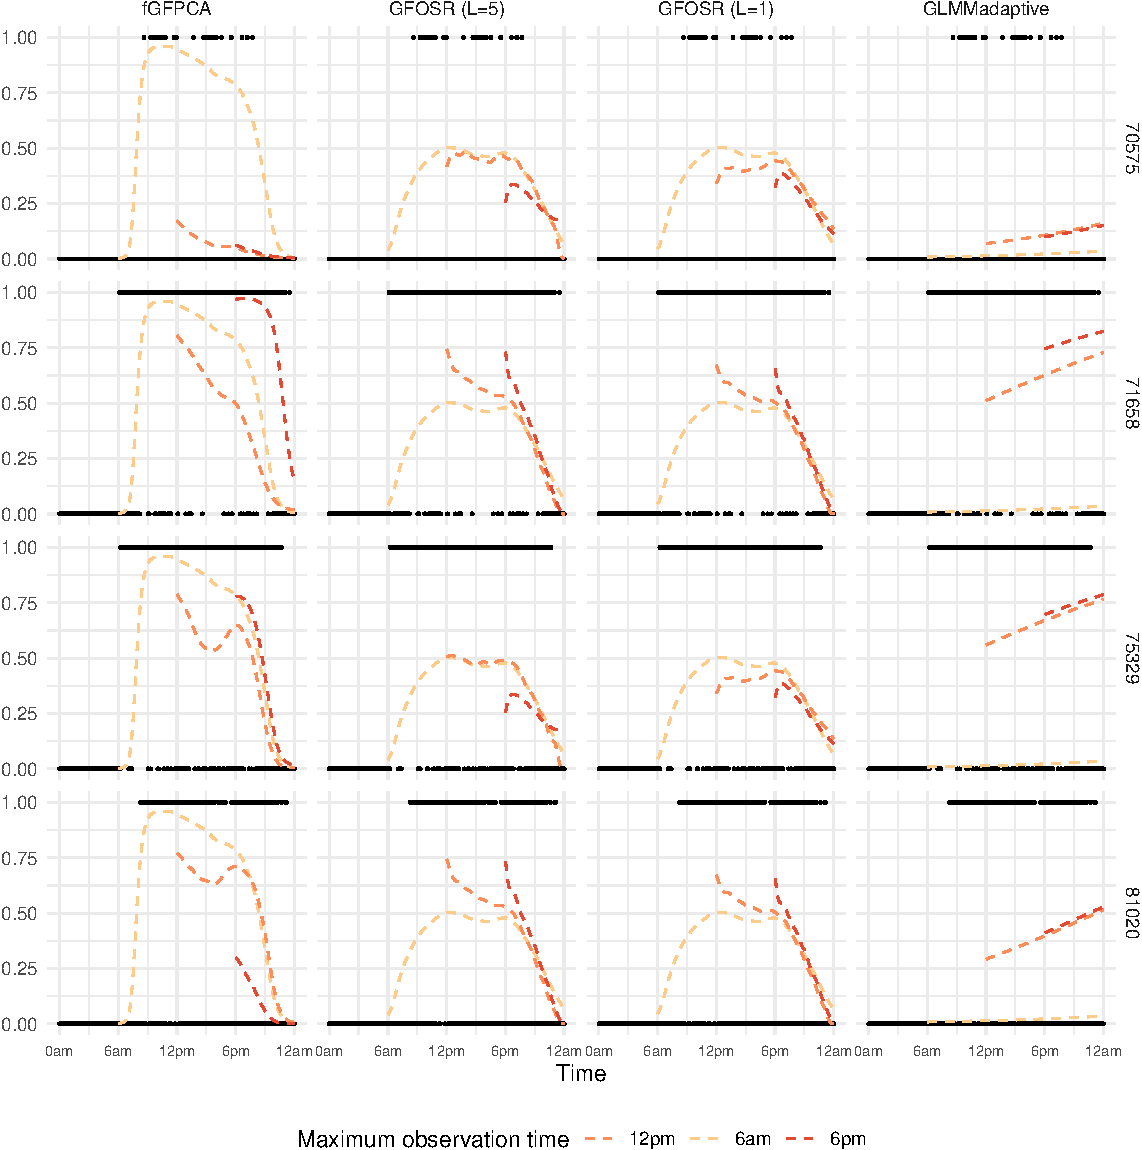
\includegraphics{manuscript_files/figure-latex/fig_appl-1.pdf}

The fGFPCA prediction conditional on observation up to 6am looks
identical across subjects. This is not due to coding issue. In fact, if
we look at individual tracks, out of 3506 subjects there are 1473 unique
predicted tracks. There is a high change the selected four subjects all
have the same predicted tracks.

PS number of unique predicted tracks is: - 3456 when conditional on 12
pm - 3488 when conditional on 6pm

I think this is closedly determined by the variety of observed outcome
across individuals. When conditioning on 6am, there are 1475 unique
observed tracks; and 3465 and 3488 respectively when obesrved up to 12pm
and 6pm. As we see, these numbers are very close to the number of unique
prediction tracks in fGFPCA.

I'd note that the four randomly selected subjects from the last report
happen to have exactly the same observations from 0-6am. That is why
they also have identical prediction after 6am. Therefore, in this report
I arbitrarily assigned subjects to be displayed: 62161, .

In addition: - For GFOSR (L5), number of unique predicted tracks are 31,
32, 32 - For GFOSR (L1), number of unique predicted tracks are 2, 2, 2 -
For GLMMadaptive, number of unique predicted tracks are 294, 712, 1533.

\begin{Shaded}
\begin{Highlighting}[]
\FunctionTok{length}\NormalTok{(}\FunctionTok{unique}\NormalTok{(pred\_nhanes\_adglmm}\SpecialCharTok{$}\NormalTok{id))}
\NormalTok{pred\_nhanes\_fgfpca }\SpecialCharTok{\%\textgreater{}\%}
  \CommentTok{\# filter(id \%in\% rand\_id) \%\textgreater{}\%}
  \FunctionTok{select}\NormalTok{(id, sind, Y) }\SpecialCharTok{\%\textgreater{}\%}
  \FunctionTok{filter}\NormalTok{(sind }\SpecialCharTok{\textless{}=}  \DecValTok{360}\NormalTok{) }\SpecialCharTok{\%\textgreater{}\%}
  \FunctionTok{pivot\_wider}\NormalTok{(}\AttributeTok{names\_from =}\NormalTok{ sind, }\AttributeTok{values\_from =}\NormalTok{ Y, }\AttributeTok{names\_prefix =} \StringTok{"sind"}\NormalTok{) }\SpecialCharTok{\%\textgreater{}\%}
  \FunctionTok{distinct}\NormalTok{(., }\FunctionTok{pick}\NormalTok{(}\FunctionTok{starts\_with}\NormalTok{(}\StringTok{"sind"}\NormalTok{)), }\AttributeTok{.keep\_all =}\NormalTok{ T) }\SpecialCharTok{\%\textgreater{}\%}
  \FunctionTok{select}\NormalTok{(id) }\SpecialCharTok{\%\textgreater{}\%}
  \FunctionTok{t}\NormalTok{() }\SpecialCharTok{\%\textgreater{}\%}
  \FunctionTok{sample}\NormalTok{(., }\AttributeTok{size =} \DecValTok{4}\NormalTok{)}


  \CommentTok{\# ggplot(aes(x=sind, y=pred360, col = as.factor(id), group = as.factor(id)))+}
  \CommentTok{\# geom\_line()}
\end{Highlighting}
\end{Shaded}

\begin{Shaded}
\begin{Highlighting}[]
\NormalTok{pred\_nhanes\_fgfpca }\SpecialCharTok{\%\textgreater{}\%}
  \FunctionTok{select}\NormalTok{(id, sind, pred360) }\SpecialCharTok{\%\textgreater{}\%}
  \FunctionTok{filter}\NormalTok{(sind}\SpecialCharTok{\textgreater{}}\DecValTok{360}\NormalTok{) }\SpecialCharTok{\%\textgreater{}\%}
  \FunctionTok{ggplot}\NormalTok{()}\SpecialCharTok{+}
  \FunctionTok{geom\_line}\NormalTok{(}\FunctionTok{aes}\NormalTok{(}\AttributeTok{x=}\NormalTok{sind, }\AttributeTok{y=}\NormalTok{pred360, }\AttributeTok{col =} \FunctionTok{as.factor}\NormalTok{(id)), }\AttributeTok{show.legend =}\NormalTok{ F)}

\NormalTok{pred\_nhanes\_fgfpca }\SpecialCharTok{\%\textgreater{}\%}
  \FunctionTok{select}\NormalTok{(id, sind, pred720) }\SpecialCharTok{\%\textgreater{}\%}
  \FunctionTok{filter}\NormalTok{(sind}\SpecialCharTok{\textgreater{}}\DecValTok{720}\NormalTok{) }\SpecialCharTok{\%\textgreater{}\%}
  \FunctionTok{ggplot}\NormalTok{()}\SpecialCharTok{+}
  \FunctionTok{geom\_line}\NormalTok{(}\FunctionTok{aes}\NormalTok{(}\AttributeTok{x=}\NormalTok{sind, }\AttributeTok{y=}\NormalTok{pred720, }\AttributeTok{col =} \FunctionTok{as.factor}\NormalTok{(id)), }\AttributeTok{show.legend =}\NormalTok{ F)}
\end{Highlighting}
\end{Shaded}

\hypertarget{additional-figures}{%
\section{Additional figures}\label{additional-figures}}

\begin{Shaded}
\begin{Highlighting}[]
\NormalTok{df\_nhanes }\OtherTok{\textless{}{-}} \FunctionTok{read\_rds}\NormalTok{(}\FunctionTok{here}\NormalTok{(}\StringTok{"Data/nhanes\_bi.rds"}\NormalTok{))}
\NormalTok{df\_nhanes }\SpecialCharTok{\%\textgreater{}\%} 
  \FunctionTok{select}\NormalTok{(SEQN, Z, sind) }\SpecialCharTok{\%\textgreater{}\%}
  \FunctionTok{filter}\NormalTok{(SEQN }\SpecialCharTok{\%in\%}\NormalTok{ rand\_id) }\SpecialCharTok{\%\textgreater{}\%}
  \FunctionTok{filter}\NormalTok{(sind }\SpecialCharTok{\%in\%} \DecValTok{356}\SpecialCharTok{:}\DecValTok{360}\NormalTok{) }\SpecialCharTok{\%\textgreater{}\%}
  \FunctionTok{pivot\_wider}\NormalTok{(}\AttributeTok{names\_from =}\NormalTok{ sind, }\AttributeTok{values\_from =}\NormalTok{ Z) }\SpecialCharTok{\%\textgreater{}\%} 
  \FunctionTok{select}\NormalTok{(}\SpecialCharTok{{-}}\NormalTok{SEQN) }\SpecialCharTok{\%\textgreater{}\%} \FunctionTok{distinct}\NormalTok{(.)}


\NormalTok{pred\_appl\_gfosr\_l5 }\SpecialCharTok{\%\textgreater{}\%} 
  \FunctionTok{filter}\NormalTok{(id }\SpecialCharTok{\%in\%}\NormalTok{ rand\_id) }\SpecialCharTok{\%\textgreater{}\%}
  \FunctionTok{select}\NormalTok{(id, sind, pred360) }\SpecialCharTok{\%\textgreater{}\%}
  \FunctionTok{pivot\_wider}\NormalTok{(}\AttributeTok{names\_from =}\NormalTok{ sind, }\AttributeTok{values\_from =}\NormalTok{ pred360) }\SpecialCharTok{\%\textgreater{}\%} 
  \FunctionTok{select}\NormalTok{(}\SpecialCharTok{{-}}\NormalTok{id) }\SpecialCharTok{\%\textgreater{}\%} \FunctionTok{distinct}\NormalTok{(.)}
\end{Highlighting}
\end{Shaded}


\end{document}
